\documentclass[twoside]{book}

% Packages required by doxygen
\usepackage{fixltx2e}
\usepackage{calc}
\usepackage{doxygen}
\usepackage{graphicx}
\usepackage[utf8]{inputenc}
\usepackage{makeidx}
\usepackage{multicol}
\usepackage{multirow}
\PassOptionsToPackage{warn}{textcomp}
\usepackage{textcomp}
\usepackage[nointegrals]{wasysym}
\usepackage[table]{xcolor}

% NLS support packages
\usepackage[swedish]{babel}

% Font selection
\usepackage[T1]{fontenc}
\usepackage{mathptmx}
\usepackage[scaled=.90]{helvet}
\usepackage{courier}
\usepackage{amssymb}
\usepackage{sectsty}
\renewcommand{\familydefault}{\sfdefault}
\allsectionsfont{%
  \fontseries{bc}\selectfont%
  \color{darkgray}%
}
\renewcommand{\DoxyLabelFont}{%
  \fontseries{bc}\selectfont%
  \color{darkgray}%
}
\newcommand{\+}{\discretionary{\mbox{\scriptsize$\hookleftarrow$}}{}{}}

% Page & text layout
\usepackage{geometry}
\geometry{%
  a4paper,%
  top=2.5cm,%
  bottom=2.5cm,%
  left=2.5cm,%
  right=2.5cm%
}
\tolerance=750
\hfuzz=15pt
\hbadness=750
\setlength{\emergencystretch}{15pt}
\setlength{\parindent}{0cm}
\setlength{\parskip}{0.2cm}
\makeatletter
\renewcommand{\paragraph}{%
  \@startsection{paragraph}{4}{0ex}{-1.0ex}{1.0ex}{%
    \normalfont\normalsize\bfseries\SS@parafont%
  }%
}
\renewcommand{\subparagraph}{%
  \@startsection{subparagraph}{5}{0ex}{-1.0ex}{1.0ex}{%
    \normalfont\normalsize\bfseries\SS@subparafont%
  }%
}
\makeatother

% Headers & footers
\usepackage{fancyhdr}
\pagestyle{fancyplain}
\fancyhead[LE]{\fancyplain{}{\bfseries\thepage}}
\fancyhead[CE]{\fancyplain{}{}}
\fancyhead[RE]{\fancyplain{}{\bfseries\leftmark}}
\fancyhead[LO]{\fancyplain{}{\bfseries\rightmark}}
\fancyhead[CO]{\fancyplain{}{}}
\fancyhead[RO]{\fancyplain{}{\bfseries\thepage}}
\fancyfoot[LE]{\fancyplain{}{}}
\fancyfoot[CE]{\fancyplain{}{}}
\fancyfoot[RE]{\fancyplain{}{\bfseries\scriptsize Skapad Mån 13 Oct 2014 17\+:17\+:58 för Livekodning 2014-\/10-\/09 I\+O\+O\+P\+M av Doxygen }}
\fancyfoot[LO]{\fancyplain{}{\bfseries\scriptsize Skapad Mån 13 Oct 2014 17\+:17\+:58 för Livekodning 2014-\/10-\/09 I\+O\+O\+P\+M av Doxygen }}
\fancyfoot[CO]{\fancyplain{}{}}
\fancyfoot[RO]{\fancyplain{}{}}
\renewcommand{\footrulewidth}{0.4pt}
\renewcommand{\chaptermark}[1]{%
  \markboth{#1}{}%
}
\renewcommand{\sectionmark}[1]{%
  \markright{\thesection\ #1}%
}

% Indices & bibliography
\usepackage{natbib}
\usepackage[titles]{tocloft}
\setcounter{tocdepth}{3}
\setcounter{secnumdepth}{5}
\makeindex

% Hyperlinks (required, but should be loaded last)
\usepackage{ifpdf}
\ifpdf
  \usepackage[pdftex,pagebackref=true]{hyperref}
\else
  \usepackage[ps2pdf,pagebackref=true]{hyperref}
\fi
\hypersetup{%
  colorlinks=true,%
  linkcolor=blue,%
  citecolor=blue,%
  unicode%
}

% Custom commands
\newcommand{\clearemptydoublepage}{%
  \newpage{\pagestyle{empty}\cleardoublepage}%
}


%===== C O N T E N T S =====

\begin{document}

% Titlepage & ToC
\hypersetup{pageanchor=false,
             bookmarks=true,
             bookmarksnumbered=true,
             pdfencoding=unicode
            }
\pagenumbering{roman}
\begin{titlepage}
\vspace*{7cm}
\begin{center}%
{\Large Livekodning 2014-\/10-\/09 I\+O\+O\+P\+M }\\
\vspace*{1cm}
{\large Skapad av Doxygen 1.8.8}\\
\vspace*{0.5cm}
{\small Mån 13 Oct 2014 17:17:58}\\
\end{center}
\end{titlepage}
\clearemptydoublepage
\tableofcontents
\clearemptydoublepage
\pagenumbering{arabic}
\hypersetup{pageanchor=true}

%--- Begin generated contents ---
\chapter{Index över datastrukturer}
\section{Datastrukturer}
Här följer datastrukturerna med korta beskrivningar\+:\begin{DoxyCompactList}
\item\contentsline{section}{\hyperlink{structkey__value}{key\+\_\+value} }{\pageref{structkey__value}}{}
\item\contentsline{section}{\hyperlink{structnode}{node} }{\pageref{structnode}}{}
\item\contentsline{section}{\hyperlink{structtree}{tree} }{\pageref{structtree}}{}
\end{DoxyCompactList}

\chapter{Filindex}
\section{Fillista}
Här följer en lista över alla filer, med en kort beskrivning\+:\begin{DoxyCompactList}
\item\contentsline{section}{tree/\hyperlink{balance_8c}{balance.\+c} }{\pageref{balance_8c}}{}
\item\contentsline{section}{tree/\hyperlink{balance_8h}{balance.\+h} }{\pageref{balance_8h}}{}
\item\contentsline{section}{tree/\hyperlink{node_8c}{node.\+c} }{\pageref{node_8c}}{}
\item\contentsline{section}{tree/\hyperlink{node_8h}{node.\+h} }{\pageref{node_8h}}{}
\item\contentsline{section}{tree/\hyperlink{tree_8c}{tree.\+c} }{\pageref{tree_8c}}{}
\item\contentsline{section}{tree/\hyperlink{tree_8h}{tree.\+h} }{\pageref{tree_8h}}{}
\item\contentsline{section}{tree/\hyperlink{util_8c}{util.\+c} }{\pageref{util_8c}}{}
\item\contentsline{section}{tree/\hyperlink{util_8h}{util.\+h} }{\pageref{util_8h}}{}
\end{DoxyCompactList}

\chapter{Dokumentation över datastrukturer}
\hypertarget{structkey__value}{\section{key\+\_\+value struktreferens}
\label{structkey__value}\index{key\+\_\+value@{key\+\_\+value}}
}


{\ttfamily \#include $<$node.\+h$>$}

\subsection*{Datafält}
\begin{DoxyCompactItemize}
\item 
void $\ast$ \hyperlink{structkey__value_a43a92ed366b412e8aa7c8a664d71e685}{key}
\item 
void $\ast$ \hyperlink{structkey__value_ae0993347bcd5222afe71d54d043f990e}{value}
\end{DoxyCompactItemize}


\subsection{Fält dokumentation}
\hypertarget{structkey__value_a43a92ed366b412e8aa7c8a664d71e685}{\index{key\+\_\+value@{key\+\_\+value}!key@{key}}
\index{key@{key}!key\+\_\+value@{key\+\_\+value}}
\subsubsection[{key}]{\setlength{\rightskip}{0pt plus 5cm}void$\ast$ key\+\_\+value\+::key}}\label{structkey__value_a43a92ed366b412e8aa7c8a664d71e685}
\hypertarget{structkey__value_ae0993347bcd5222afe71d54d043f990e}{\index{key\+\_\+value@{key\+\_\+value}!value@{value}}
\index{value@{value}!key\+\_\+value@{key\+\_\+value}}
\subsubsection[{value}]{\setlength{\rightskip}{0pt plus 5cm}void$\ast$ key\+\_\+value\+::value}}\label{structkey__value_ae0993347bcd5222afe71d54d043f990e}


Dokumentationen för denna strukt var genererad från följande fil\+:\begin{DoxyCompactItemize}
\item 
tree/\hyperlink{node_8h}{node.\+h}\end{DoxyCompactItemize}

\hypertarget{structnode}{\section{node struktreferens}
\label{structnode}\index{node@{node}}
}


{\ttfamily \#include $<$node.\+h$>$}



Samarbetsdiagram för node\+:
\nopagebreak
\begin{figure}[H]
\begin{center}
\leavevmode
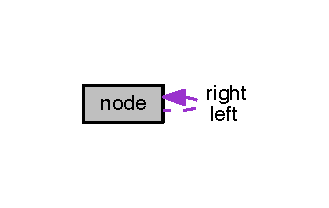
\includegraphics[width=158pt]{structnode__coll__graph}
\end{center}
\end{figure}
\subsection*{Datafält}
\begin{DoxyCompactItemize}
\item 
struct \hyperlink{structnode}{node} $\ast$ \hyperlink{structnode_a3ce38490a651bfda86d88ff955e96abc}{left}
\item 
struct \hyperlink{structnode}{node} $\ast$ \hyperlink{structnode_a875f75abfe22103500535b179828e4e3}{right}
\item 
void $\ast$ \hyperlink{structnode_a72c8a0c41b801c92db89c5078642f28b}{key}
\item 
void $\ast$ \hyperlink{structnode_a288a44aecd04d7839824d50a0b65982e}{value}
\end{DoxyCompactItemize}


\subsection{Fält dokumentation}
\hypertarget{structnode_a72c8a0c41b801c92db89c5078642f28b}{\index{node@{node}!key@{key}}
\index{key@{key}!node@{node}}
\subsubsection[{key}]{\setlength{\rightskip}{0pt plus 5cm}void$\ast$ node\+::key}}\label{structnode_a72c8a0c41b801c92db89c5078642f28b}
\hypertarget{structnode_a3ce38490a651bfda86d88ff955e96abc}{\index{node@{node}!left@{left}}
\index{left@{left}!node@{node}}
\subsubsection[{left}]{\setlength{\rightskip}{0pt plus 5cm}struct {\bf node}$\ast$ node\+::left}}\label{structnode_a3ce38490a651bfda86d88ff955e96abc}
\hypertarget{structnode_a875f75abfe22103500535b179828e4e3}{\index{node@{node}!right@{right}}
\index{right@{right}!node@{node}}
\subsubsection[{right}]{\setlength{\rightskip}{0pt plus 5cm}struct {\bf node}$\ast$ node\+::right}}\label{structnode_a875f75abfe22103500535b179828e4e3}
\hypertarget{structnode_a288a44aecd04d7839824d50a0b65982e}{\index{node@{node}!value@{value}}
\index{value@{value}!node@{node}}
\subsubsection[{value}]{\setlength{\rightskip}{0pt plus 5cm}void$\ast$ node\+::value}}\label{structnode_a288a44aecd04d7839824d50a0b65982e}


Dokumentationen för denna strukt var genererad från följande fil\+:\begin{DoxyCompactItemize}
\item 
tree/\hyperlink{node_8h}{node.\+h}\end{DoxyCompactItemize}

\hypertarget{structtree}{\section{tree struktreferens}
\label{structtree}\index{tree@{tree}}
}


Samarbetsdiagram för tree\+:
\nopagebreak
\begin{figure}[H]
\begin{center}
\leavevmode
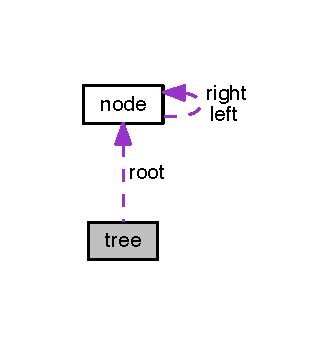
\includegraphics[width=158pt]{structtree__coll__graph}
\end{center}
\end{figure}
\subsection*{Datafält}
\begin{DoxyCompactItemize}
\item 
\hyperlink{node_8h_aeed67813c57d1b99aba54f16aa01639f}{node\+\_\+s} $\ast$ \hyperlink{structtree_a752f44752a2b0a0ba6fb3f434d7feea6}{root}
\item 
\hyperlink{tree_8h_ac9404bce0090a72ec95c26c1fc58e4dd}{cmp\+\_\+f} \hyperlink{structtree_ad2c95bd73b4c3f1ace5705b380c971cb}{key\+\_\+cmp}
\item 
bool \hyperlink{structtree_a71c5140877d3e8978670898bfb87cb07}{should\+\_\+balance}
\end{DoxyCompactItemize}


\subsection{Fält dokumentation}
\hypertarget{structtree_ad2c95bd73b4c3f1ace5705b380c971cb}{\index{tree@{tree}!key\+\_\+cmp@{key\+\_\+cmp}}
\index{key\+\_\+cmp@{key\+\_\+cmp}!tree@{tree}}
\subsubsection[{key\+\_\+cmp}]{\setlength{\rightskip}{0pt plus 5cm}{\bf cmp\+\_\+f} tree\+::key\+\_\+cmp}}\label{structtree_ad2c95bd73b4c3f1ace5705b380c971cb}
\hypertarget{structtree_a752f44752a2b0a0ba6fb3f434d7feea6}{\index{tree@{tree}!root@{root}}
\index{root@{root}!tree@{tree}}
\subsubsection[{root}]{\setlength{\rightskip}{0pt plus 5cm}{\bf node\+\_\+s}$\ast$ tree\+::root}}\label{structtree_a752f44752a2b0a0ba6fb3f434d7feea6}
\hypertarget{structtree_a71c5140877d3e8978670898bfb87cb07}{\index{tree@{tree}!should\+\_\+balance@{should\+\_\+balance}}
\index{should\+\_\+balance@{should\+\_\+balance}!tree@{tree}}
\subsubsection[{should\+\_\+balance}]{\setlength{\rightskip}{0pt plus 5cm}bool tree\+::should\+\_\+balance}}\label{structtree_a71c5140877d3e8978670898bfb87cb07}


Dokumentationen för denna strukt var genererad från följande fil\+:\begin{DoxyCompactItemize}
\item 
tree/\hyperlink{tree_8c}{tree.\+c}\end{DoxyCompactItemize}

\chapter{Dokumentation över filer}
\hypertarget{balance_8c}{\section{tree/balance.c filreferens}
\label{balance_8c}\index{tree/balance.\+c@{tree/balance.\+c}}
}
{\ttfamily \#include $<$stdlib.\+h$>$}\\*
{\ttfamily \#include $<$stdint.\+h$>$}\\*
{\ttfamily \#include \char`\"{}balance.\+h\char`\"{}}\\*
{\ttfamily \#include \char`\"{}node.\+h\char`\"{}}\\*
Include-\/beroendediagram för balance.\+c\+:
\nopagebreak
\begin{figure}[H]
\begin{center}
\leavevmode
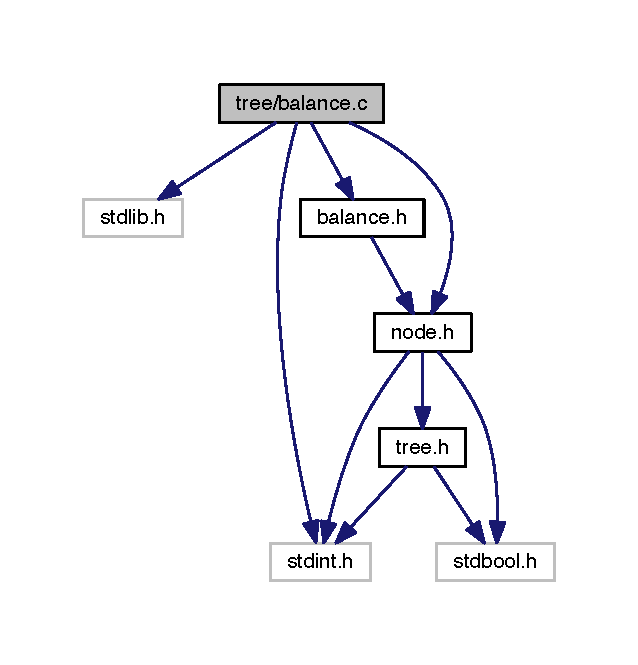
\includegraphics[width=306pt]{balance_8c__incl}
\end{center}
\end{figure}
\subsection*{Egenuppräknande typer}
\begin{DoxyCompactItemize}
\item 
enum \hyperlink{balance_8c_a1e7ef09ce66d09456a55c47a8c42f3dc}{balance} \{ \\*
\hyperlink{balance_8c_a1e7ef09ce66d09456a55c47a8c42f3dcae08ac5ba637bc42d8e480e5d70337a89}{B\+A\+L\+A\+N\+C\+E\+D}, 
\hyperlink{balance_8c_a1e7ef09ce66d09456a55c47a8c42f3dca5c6ec9e8eb3d749c847feba2008c0d51}{L\+E\+F\+T\+\_\+\+L\+E\+F\+T\+\_\+\+H\+E\+A\+V\+Y}, 
\hyperlink{balance_8c_a1e7ef09ce66d09456a55c47a8c42f3dcad0767e89e28375ca9044e1c3d313331b}{L\+E\+F\+T\+\_\+\+R\+I\+G\+H\+T\+\_\+\+H\+E\+A\+V\+Y}, 
\hyperlink{balance_8c_a1e7ef09ce66d09456a55c47a8c42f3dca599662d20189f9cd96ff2e1f5bd48816}{R\+I\+G\+H\+T\+\_\+\+L\+E\+F\+T\+\_\+\+H\+E\+A\+V\+Y}, 
\\*
\hyperlink{balance_8c_a1e7ef09ce66d09456a55c47a8c42f3dca7881fb0f0738fb8dda2f277cd6a60ddc}{R\+I\+G\+H\+T\+\_\+\+R\+I\+G\+H\+T\+\_\+\+H\+E\+A\+V\+Y}
 \}
\end{DoxyCompactItemize}
\subsection*{Funktioner}
\begin{DoxyCompactItemize}
\item 
\hyperlink{node_8h_aeed67813c57d1b99aba54f16aa01639f}{node\+\_\+s} $\ast$ \hyperlink{balance_8c_a499050d5573d5070a0973a56dac79315}{rotate\+\_\+left} (\hyperlink{node_8h_aeed67813c57d1b99aba54f16aa01639f}{node\+\_\+s} $\ast$n)
\item 
\hyperlink{node_8h_aeed67813c57d1b99aba54f16aa01639f}{node\+\_\+s} $\ast$ \hyperlink{balance_8c_a536da07b68b69d0131501f54ec2def6a}{flip\+\_\+left} (\hyperlink{node_8h_aeed67813c57d1b99aba54f16aa01639f}{node\+\_\+s} $\ast$n)
\item 
\hyperlink{node_8h_aeed67813c57d1b99aba54f16aa01639f}{node\+\_\+s} $\ast$ \hyperlink{balance_8c_a55c8417a5335da0856e7f5b1feaa636f}{rotate\+\_\+right} (\hyperlink{node_8h_aeed67813c57d1b99aba54f16aa01639f}{node\+\_\+s} $\ast$n)
\item 
\hyperlink{node_8h_aeed67813c57d1b99aba54f16aa01639f}{node\+\_\+s} $\ast$ \hyperlink{balance_8c_a6361650730a57c352dd71a4ba360fd87}{flip\+\_\+right} (\hyperlink{node_8h_aeed67813c57d1b99aba54f16aa01639f}{node\+\_\+s} $\ast$n)
\item 
enum \hyperlink{balance_8c_a1e7ef09ce66d09456a55c47a8c42f3dc}{balance} \hyperlink{balance_8c_adf0f756ba133afb0ede202ea2d39385e}{balance\+\_\+check} (\hyperlink{node_8h_aeed67813c57d1b99aba54f16aa01639f}{node\+\_\+s} $\ast$n)
\begin{DoxyCompactList}\small\item\em Kontrollerar hur välbalanserat ett subträd är. \end{DoxyCompactList}\item 
void \hyperlink{balance_8c_a2689da611315fb6d26133997568c32e3}{balance\+\_\+subtree} (\hyperlink{node_8h_aeed67813c57d1b99aba54f16aa01639f}{node\+\_\+s} $\ast$$\ast$$\ast$ns, uint32\+\_\+t ns\+\_\+size)
\end{DoxyCompactItemize}


\subsection{Dokumentation över egenuppräknande typer}
\hypertarget{balance_8c_a1e7ef09ce66d09456a55c47a8c42f3dc}{\index{balance.\+c@{balance.\+c}!balance@{balance}}
\index{balance@{balance}!balance.\+c@{balance.\+c}}
\subsubsection[{balance}]{\setlength{\rightskip}{0pt plus 5cm}enum {\bf balance}}}\label{balance_8c_a1e7ef09ce66d09456a55c47a8c42f3dc}
\begin{Desc}
\item[Egenuppräknade typers värden]\par
\begin{description}
\index{B\+A\+L\+A\+N\+C\+E\+D@{B\+A\+L\+A\+N\+C\+E\+D}!balance.\+c@{balance.\+c}}\index{balance.\+c@{balance.\+c}!B\+A\+L\+A\+N\+C\+E\+D@{B\+A\+L\+A\+N\+C\+E\+D}}\item[{\em 
\hypertarget{balance_8c_a1e7ef09ce66d09456a55c47a8c42f3dcae08ac5ba637bc42d8e480e5d70337a89}{B\+A\+L\+A\+N\+C\+E\+D}\label{balance_8c_a1e7ef09ce66d09456a55c47a8c42f3dcae08ac5ba637bc42d8e480e5d70337a89}
}]\index{L\+E\+F\+T\+\_\+\+L\+E\+F\+T\+\_\+\+H\+E\+A\+V\+Y@{L\+E\+F\+T\+\_\+\+L\+E\+F\+T\+\_\+\+H\+E\+A\+V\+Y}!balance.\+c@{balance.\+c}}\index{balance.\+c@{balance.\+c}!L\+E\+F\+T\+\_\+\+L\+E\+F\+T\+\_\+\+H\+E\+A\+V\+Y@{L\+E\+F\+T\+\_\+\+L\+E\+F\+T\+\_\+\+H\+E\+A\+V\+Y}}\item[{\em 
\hypertarget{balance_8c_a1e7ef09ce66d09456a55c47a8c42f3dca5c6ec9e8eb3d749c847feba2008c0d51}{L\+E\+F\+T\+\_\+\+L\+E\+F\+T\+\_\+\+H\+E\+A\+V\+Y}\label{balance_8c_a1e7ef09ce66d09456a55c47a8c42f3dca5c6ec9e8eb3d749c847feba2008c0d51}
}]\index{L\+E\+F\+T\+\_\+\+R\+I\+G\+H\+T\+\_\+\+H\+E\+A\+V\+Y@{L\+E\+F\+T\+\_\+\+R\+I\+G\+H\+T\+\_\+\+H\+E\+A\+V\+Y}!balance.\+c@{balance.\+c}}\index{balance.\+c@{balance.\+c}!L\+E\+F\+T\+\_\+\+R\+I\+G\+H\+T\+\_\+\+H\+E\+A\+V\+Y@{L\+E\+F\+T\+\_\+\+R\+I\+G\+H\+T\+\_\+\+H\+E\+A\+V\+Y}}\item[{\em 
\hypertarget{balance_8c_a1e7ef09ce66d09456a55c47a8c42f3dcad0767e89e28375ca9044e1c3d313331b}{L\+E\+F\+T\+\_\+\+R\+I\+G\+H\+T\+\_\+\+H\+E\+A\+V\+Y}\label{balance_8c_a1e7ef09ce66d09456a55c47a8c42f3dcad0767e89e28375ca9044e1c3d313331b}
}]\index{R\+I\+G\+H\+T\+\_\+\+L\+E\+F\+T\+\_\+\+H\+E\+A\+V\+Y@{R\+I\+G\+H\+T\+\_\+\+L\+E\+F\+T\+\_\+\+H\+E\+A\+V\+Y}!balance.\+c@{balance.\+c}}\index{balance.\+c@{balance.\+c}!R\+I\+G\+H\+T\+\_\+\+L\+E\+F\+T\+\_\+\+H\+E\+A\+V\+Y@{R\+I\+G\+H\+T\+\_\+\+L\+E\+F\+T\+\_\+\+H\+E\+A\+V\+Y}}\item[{\em 
\hypertarget{balance_8c_a1e7ef09ce66d09456a55c47a8c42f3dca599662d20189f9cd96ff2e1f5bd48816}{R\+I\+G\+H\+T\+\_\+\+L\+E\+F\+T\+\_\+\+H\+E\+A\+V\+Y}\label{balance_8c_a1e7ef09ce66d09456a55c47a8c42f3dca599662d20189f9cd96ff2e1f5bd48816}
}]\index{R\+I\+G\+H\+T\+\_\+\+R\+I\+G\+H\+T\+\_\+\+H\+E\+A\+V\+Y@{R\+I\+G\+H\+T\+\_\+\+R\+I\+G\+H\+T\+\_\+\+H\+E\+A\+V\+Y}!balance.\+c@{balance.\+c}}\index{balance.\+c@{balance.\+c}!R\+I\+G\+H\+T\+\_\+\+R\+I\+G\+H\+T\+\_\+\+H\+E\+A\+V\+Y@{R\+I\+G\+H\+T\+\_\+\+R\+I\+G\+H\+T\+\_\+\+H\+E\+A\+V\+Y}}\item[{\em 
\hypertarget{balance_8c_a1e7ef09ce66d09456a55c47a8c42f3dca7881fb0f0738fb8dda2f277cd6a60ddc}{R\+I\+G\+H\+T\+\_\+\+R\+I\+G\+H\+T\+\_\+\+H\+E\+A\+V\+Y}\label{balance_8c_a1e7ef09ce66d09456a55c47a8c42f3dca7881fb0f0738fb8dda2f277cd6a60ddc}
}]\end{description}
\end{Desc}


\subsection{Dokumentation över funktioner}
\hypertarget{balance_8c_adf0f756ba133afb0ede202ea2d39385e}{\index{balance.\+c@{balance.\+c}!balance\+\_\+check@{balance\+\_\+check}}
\index{balance\+\_\+check@{balance\+\_\+check}!balance.\+c@{balance.\+c}}
\subsubsection[{balance\+\_\+check}]{\setlength{\rightskip}{0pt plus 5cm}enum {\bf balance} balance\+\_\+check (
\begin{DoxyParamCaption}
\item[{{\bf node\+\_\+s} $\ast$}]{n}
\end{DoxyParamCaption}
)}}\label{balance_8c_adf0f756ba133afb0ede202ea2d39385e}


Kontrollerar hur välbalanserat ett subträd är. 

\begin{DoxySeeAlso}{Se även}
enum \hyperlink{balance_8c_a1e7ef09ce66d09456a55c47a8c42f3dc}{balance} 
\end{DoxySeeAlso}


Här är anropnings diagrammet för den här funktionen\+:
\nopagebreak
\begin{figure}[H]
\begin{center}
\leavevmode
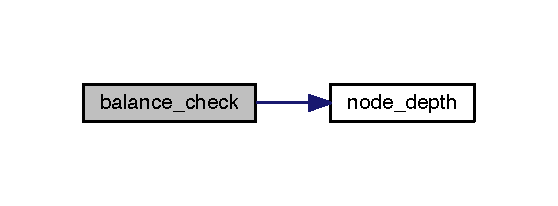
\includegraphics[width=268pt]{balance_8c_adf0f756ba133afb0ede202ea2d39385e_cgraph}
\end{center}
\end{figure}




Här är katalog-\/grafen för denna funktion\+:
\nopagebreak
\begin{figure}[H]
\begin{center}
\leavevmode
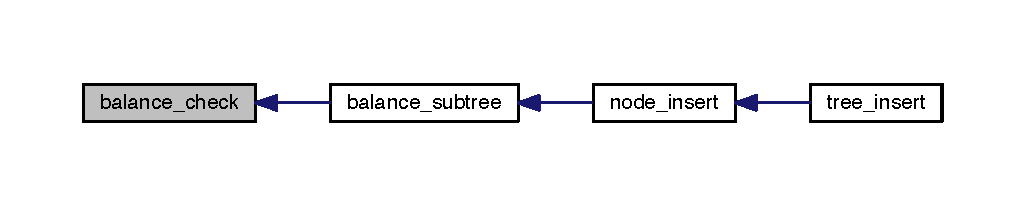
\includegraphics[width=350pt]{balance_8c_adf0f756ba133afb0ede202ea2d39385e_icgraph}
\end{center}
\end{figure}


\hypertarget{balance_8c_a2689da611315fb6d26133997568c32e3}{\index{balance.\+c@{balance.\+c}!balance\+\_\+subtree@{balance\+\_\+subtree}}
\index{balance\+\_\+subtree@{balance\+\_\+subtree}!balance.\+c@{balance.\+c}}
\subsubsection[{balance\+\_\+subtree}]{\setlength{\rightskip}{0pt plus 5cm}void balance\+\_\+subtree (
\begin{DoxyParamCaption}
\item[{{\bf node\+\_\+s} $\ast$$\ast$$\ast$}]{ns, }
\item[{uint32\+\_\+t}]{ns\+\_\+size}
\end{DoxyParamCaption}
)}}\label{balance_8c_a2689da611315fb6d26133997568c32e3}


Här är anropnings diagrammet för den här funktionen\+:
\nopagebreak
\begin{figure}[H]
\begin{center}
\leavevmode
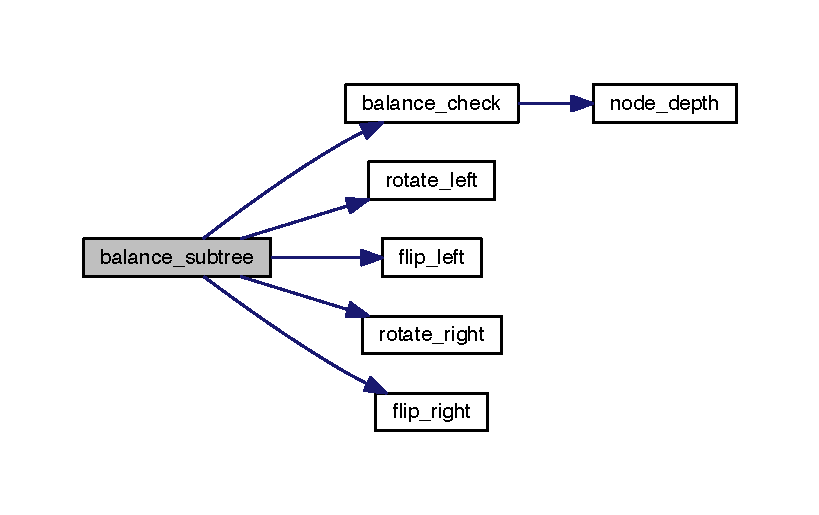
\includegraphics[width=350pt]{balance_8c_a2689da611315fb6d26133997568c32e3_cgraph}
\end{center}
\end{figure}




Här är katalog-\/grafen för denna funktion\+:
\nopagebreak
\begin{figure}[H]
\begin{center}
\leavevmode
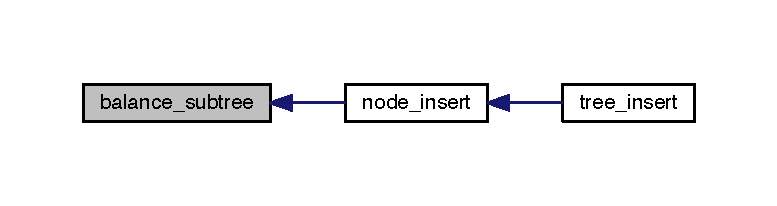
\includegraphics[width=350pt]{balance_8c_a2689da611315fb6d26133997568c32e3_icgraph}
\end{center}
\end{figure}


\hypertarget{balance_8c_a536da07b68b69d0131501f54ec2def6a}{\index{balance.\+c@{balance.\+c}!flip\+\_\+left@{flip\+\_\+left}}
\index{flip\+\_\+left@{flip\+\_\+left}!balance.\+c@{balance.\+c}}
\subsubsection[{flip\+\_\+left}]{\setlength{\rightskip}{0pt plus 5cm}{\bf node\+\_\+s} $\ast$ flip\+\_\+left (
\begin{DoxyParamCaption}
\item[{{\bf node\+\_\+s} $\ast$}]{n}
\end{DoxyParamCaption}
)}}\label{balance_8c_a536da07b68b69d0131501f54ec2def6a}


Här är katalog-\/grafen för denna funktion\+:
\nopagebreak
\begin{figure}[H]
\begin{center}
\leavevmode
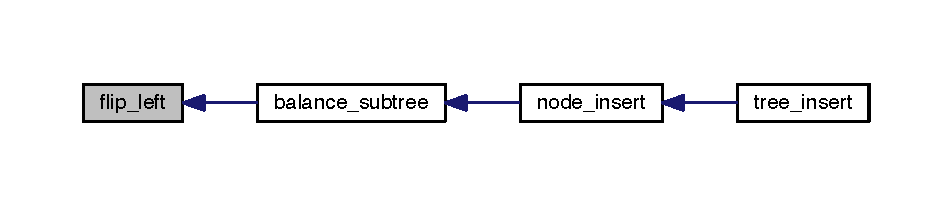
\includegraphics[width=350pt]{balance_8c_a536da07b68b69d0131501f54ec2def6a_icgraph}
\end{center}
\end{figure}


\hypertarget{balance_8c_a6361650730a57c352dd71a4ba360fd87}{\index{balance.\+c@{balance.\+c}!flip\+\_\+right@{flip\+\_\+right}}
\index{flip\+\_\+right@{flip\+\_\+right}!balance.\+c@{balance.\+c}}
\subsubsection[{flip\+\_\+right}]{\setlength{\rightskip}{0pt plus 5cm}{\bf node\+\_\+s} $\ast$ flip\+\_\+right (
\begin{DoxyParamCaption}
\item[{{\bf node\+\_\+s} $\ast$}]{n}
\end{DoxyParamCaption}
)}}\label{balance_8c_a6361650730a57c352dd71a4ba360fd87}


Här är katalog-\/grafen för denna funktion\+:
\nopagebreak
\begin{figure}[H]
\begin{center}
\leavevmode
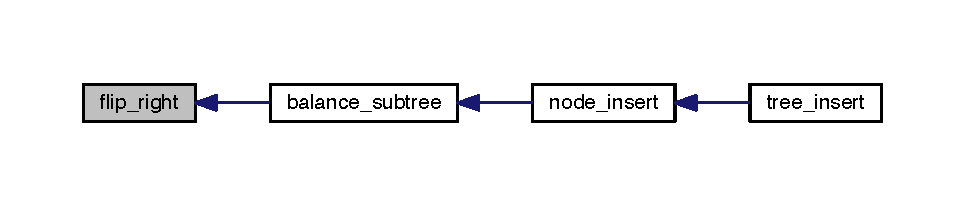
\includegraphics[width=350pt]{balance_8c_a6361650730a57c352dd71a4ba360fd87_icgraph}
\end{center}
\end{figure}


\hypertarget{balance_8c_a499050d5573d5070a0973a56dac79315}{\index{balance.\+c@{balance.\+c}!rotate\+\_\+left@{rotate\+\_\+left}}
\index{rotate\+\_\+left@{rotate\+\_\+left}!balance.\+c@{balance.\+c}}
\subsubsection[{rotate\+\_\+left}]{\setlength{\rightskip}{0pt plus 5cm}{\bf node\+\_\+s} $\ast$ rotate\+\_\+left (
\begin{DoxyParamCaption}
\item[{{\bf node\+\_\+s} $\ast$}]{n}
\end{DoxyParamCaption}
)}}\label{balance_8c_a499050d5573d5070a0973a56dac79315}


Här är katalog-\/grafen för denna funktion\+:
\nopagebreak
\begin{figure}[H]
\begin{center}
\leavevmode
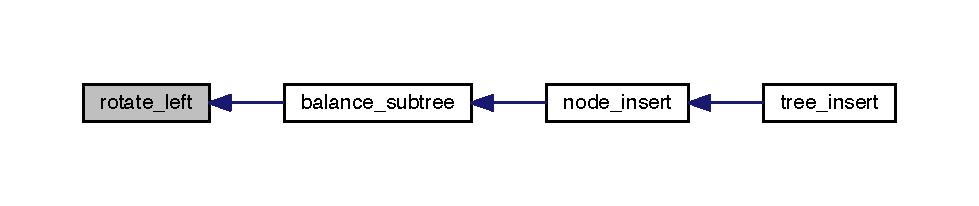
\includegraphics[width=350pt]{balance_8c_a499050d5573d5070a0973a56dac79315_icgraph}
\end{center}
\end{figure}


\hypertarget{balance_8c_a55c8417a5335da0856e7f5b1feaa636f}{\index{balance.\+c@{balance.\+c}!rotate\+\_\+right@{rotate\+\_\+right}}
\index{rotate\+\_\+right@{rotate\+\_\+right}!balance.\+c@{balance.\+c}}
\subsubsection[{rotate\+\_\+right}]{\setlength{\rightskip}{0pt plus 5cm}{\bf node\+\_\+s} $\ast$ rotate\+\_\+right (
\begin{DoxyParamCaption}
\item[{{\bf node\+\_\+s} $\ast$}]{n}
\end{DoxyParamCaption}
)}}\label{balance_8c_a55c8417a5335da0856e7f5b1feaa636f}


Här är katalog-\/grafen för denna funktion\+:
\nopagebreak
\begin{figure}[H]
\begin{center}
\leavevmode
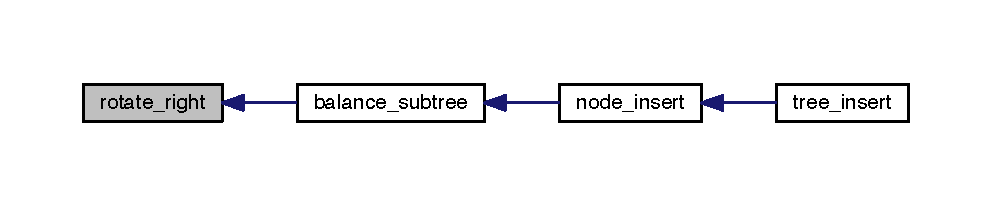
\includegraphics[width=350pt]{balance_8c_a55c8417a5335da0856e7f5b1feaa636f_icgraph}
\end{center}
\end{figure}



\hypertarget{balance_8h}{\section{tree/balance.h filreferens}
\label{balance_8h}\index{tree/balance.\+h@{tree/balance.\+h}}
}
{\ttfamily \#include \char`\"{}node.\+h\char`\"{}}\\*
Include-\/beroendediagram för balance.\+h\+:
\nopagebreak
\begin{figure}[H]
\begin{center}
\leavevmode
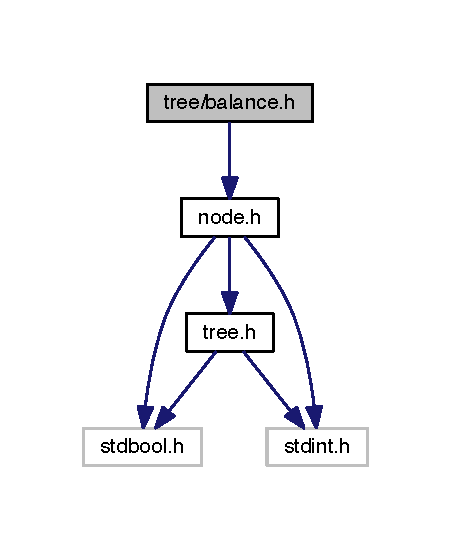
\includegraphics[width=216pt]{balance_8h__incl}
\end{center}
\end{figure}
Den här grafen visar vilka filer som direkt eller indirekt inkluderar denna filen.
\nopagebreak
\begin{figure}[H]
\begin{center}
\leavevmode
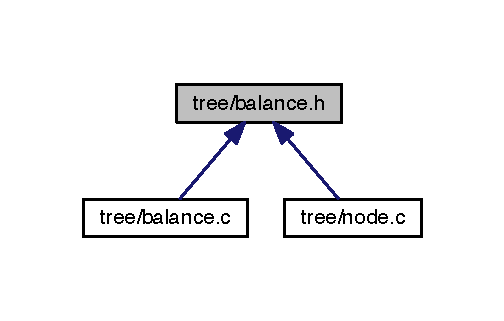
\includegraphics[width=242pt]{balance_8h__dep__incl}
\end{center}
\end{figure}
\subsection*{Funktioner}
\begin{DoxyCompactItemize}
\item 
enum \hyperlink{balance_8c_a1e7ef09ce66d09456a55c47a8c42f3dc}{balance} \hyperlink{balance_8h_adf0f756ba133afb0ede202ea2d39385e}{balance\+\_\+check} (\hyperlink{node_8h_aeed67813c57d1b99aba54f16aa01639f}{node\+\_\+s} $\ast$n)
\begin{DoxyCompactList}\small\item\em Kontrollerar hur välbalanserat ett subträd är. \end{DoxyCompactList}\item 
void \hyperlink{balance_8h_acaf035612109b377e873e7714fc61c1b}{balance\+\_\+subtree} (\hyperlink{node_8h_aeed67813c57d1b99aba54f16aa01639f}{node\+\_\+s} $\ast$$\ast$ns\mbox{[}$\,$\mbox{]}, uint32\+\_\+t ns\+\_\+size)
\end{DoxyCompactItemize}


\subsection{Dokumentation över funktioner}
\hypertarget{balance_8h_adf0f756ba133afb0ede202ea2d39385e}{\index{balance.\+h@{balance.\+h}!balance\+\_\+check@{balance\+\_\+check}}
\index{balance\+\_\+check@{balance\+\_\+check}!balance.\+h@{balance.\+h}}
\subsubsection[{balance\+\_\+check}]{\setlength{\rightskip}{0pt plus 5cm}enum {\bf balance} balance\+\_\+check (
\begin{DoxyParamCaption}
\item[{{\bf node\+\_\+s} $\ast$}]{n}
\end{DoxyParamCaption}
)}}\label{balance_8h_adf0f756ba133afb0ede202ea2d39385e}


Kontrollerar hur välbalanserat ett subträd är. 

\begin{DoxySeeAlso}{Se även}
enum \hyperlink{balance_8c_a1e7ef09ce66d09456a55c47a8c42f3dc}{balance} 
\end{DoxySeeAlso}


Här är anropnings diagrammet för den här funktionen\+:
\nopagebreak
\begin{figure}[H]
\begin{center}
\leavevmode
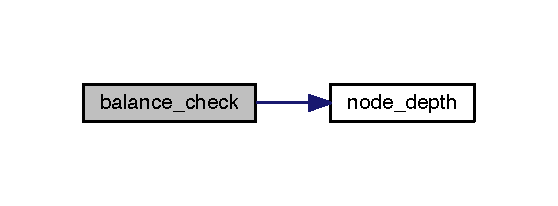
\includegraphics[width=268pt]{balance_8h_adf0f756ba133afb0ede202ea2d39385e_cgraph}
\end{center}
\end{figure}




Här är katalog-\/grafen för denna funktion\+:
\nopagebreak
\begin{figure}[H]
\begin{center}
\leavevmode
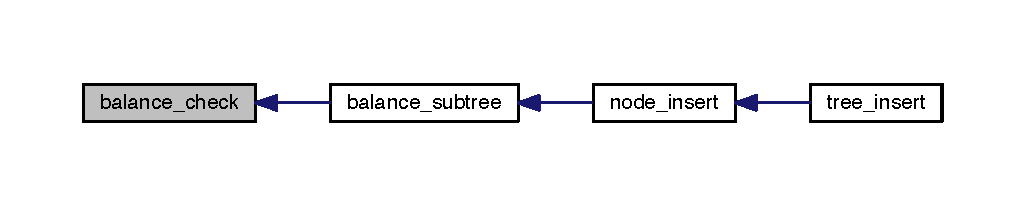
\includegraphics[width=350pt]{balance_8h_adf0f756ba133afb0ede202ea2d39385e_icgraph}
\end{center}
\end{figure}


\hypertarget{balance_8h_acaf035612109b377e873e7714fc61c1b}{\index{balance.\+h@{balance.\+h}!balance\+\_\+subtree@{balance\+\_\+subtree}}
\index{balance\+\_\+subtree@{balance\+\_\+subtree}!balance.\+h@{balance.\+h}}
\subsubsection[{balance\+\_\+subtree}]{\setlength{\rightskip}{0pt plus 5cm}void balance\+\_\+subtree (
\begin{DoxyParamCaption}
\item[{{\bf node\+\_\+s} $\ast$$\ast$}]{ns\mbox{[}$\,$\mbox{]}, }
\item[{uint32\+\_\+t}]{ns\+\_\+size}
\end{DoxyParamCaption}
)}}\label{balance_8h_acaf035612109b377e873e7714fc61c1b}
Utför 0 till {\ttfamily ns\+\_\+size} ombalanseringar av subträd rotade i {\ttfamily $\ast$ns\mbox{[}0..ns\+\_\+size-\/1\mbox{]}}.


\begin{DoxyParams}{Parametrar}
{\em ns} & en array av pekare till pekare till noder (se exempel) \\
\hline
{\em ns\+\_\+size} & storleken på {\ttfamily ns}\\
\hline
\end{DoxyParams}
Låt {\ttfamily ns == \mbox{[}p1, p2, p3\mbox{]}} när {\ttfamily ns\+\_\+size == 3}. Då skall gälla att antingen {\ttfamily \&(($\ast$p1)-\/$>$left) == p2} eller {\ttfamily \&(($\ast$p1)-\/$>$right == p2)}, och antingen {\ttfamily \&(($\ast$p2)-\/$>$left) == p3} eller {\ttfamily \&(($\ast$p2)-\/$>$right == p3)}. 
\hypertarget{node_8c}{\section{tree/node.c filreferens}
\label{node_8c}\index{tree/node.\+c@{tree/node.\+c}}
}
{\ttfamily \#include $<$stdlib.\+h$>$}\\*
{\ttfamily \#include $<$stdbool.\+h$>$}\\*
{\ttfamily \#include $<$assert.\+h$>$}\\*
{\ttfamily \#include \char`\"{}tree.\+h\char`\"{}}\\*
{\ttfamily \#include \char`\"{}node.\+h\char`\"{}}\\*
{\ttfamily \#include \char`\"{}balance.\+h\char`\"{}}\\*
Include-\/beroendediagram för node.\+c\+:
\nopagebreak
\begin{figure}[H]
\begin{center}
\leavevmode
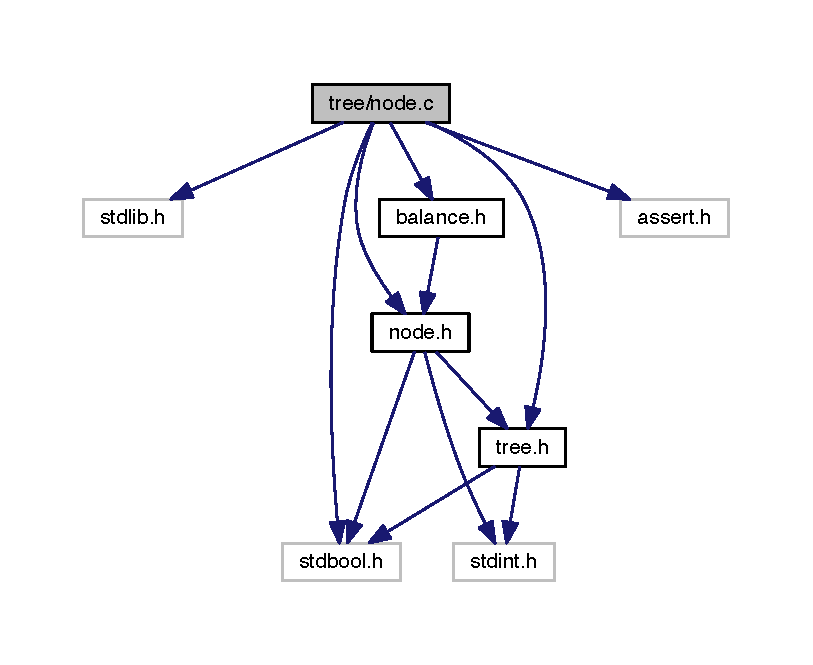
\includegraphics[width=350pt]{node_8c__incl}
\end{center}
\end{figure}
\subsection*{Definitioner}
\begin{DoxyCompactItemize}
\item 
\#define \hyperlink{node_8c_a1862ef0c9ccba20e371c3e720bbff500}{Call}(f, a1, a2)~do \{ if (a1) f(a1,a2); else f(a2,N\+U\+L\+L); \} while(0)
\item 
\#define \hyperlink{node_8c_a61555d5d1e996c64b8e49fc367660ccf}{Val\+\_\+or\+\_\+whole}(n, i)~((i) ? n \+: n-\/$>$value)
\end{DoxyCompactItemize}
\subsection*{Funktioner}
\begin{DoxyCompactItemize}
\item 
\hyperlink{node_8h_aeed67813c57d1b99aba54f16aa01639f}{node\+\_\+s} $\ast$ \hyperlink{node_8c_a51b804eb853b5938a60dbe0df42b474a}{node\+\_\+new} (void $\ast$k, void $\ast$v)
\item 
struct \hyperlink{structkey__value}{key\+\_\+value} \hyperlink{node_8c_ae1d068c29b1634d5d867c9837fc666d5}{node\+\_\+delete} (\hyperlink{node_8h_aeed67813c57d1b99aba54f16aa01639f}{node\+\_\+s} $\ast$n)
\begin{DoxyCompactList}\small\item\em Tar bort en nod ur minnet och returnerar en pekare till dess element. \end{DoxyCompactList}\item 
struct \hyperlink{structkey__value}{key\+\_\+value} \hyperlink{node_8c_a2d121428f77a50dbda46a08eeec930fd}{unlink\+\_\+smallest} (\hyperlink{node_8h_aeed67813c57d1b99aba54f16aa01639f}{node\+\_\+s} $\ast$$\ast$n)
\item 
void \hyperlink{node_8c_a9b008ff5bff9290e7d12f61ee6fe0306}{node\+\_\+insert} (\hyperlink{tree_8h_ac9404bce0090a72ec95c26c1fc58e4dd}{cmp\+\_\+f} key\+\_\+cmp, void $\ast$k, void $\ast$v, \hyperlink{node_8h_aeed67813c57d1b99aba54f16aa01639f}{node\+\_\+s} $\ast$$\ast$n, bool \hyperlink{balance_8c_a1e7ef09ce66d09456a55c47a8c42f3dc}{balance})
\begin{DoxyCompactList}\small\item\em Stoppar in ett nytt element i trädet. \end{DoxyCompactList}\item 
void \hyperlink{node_8c_a54482a8cdcd1d716d098fb8e759e5a56}{node\+\_\+traversal} (enum \hyperlink{tree_8h_a9f4e8630516f3da89537313b4c828759}{order} \hyperlink{tree_8h_a9f4e8630516f3da89537313b4c828759}{order}, \hyperlink{node_8h_aeed67813c57d1b99aba54f16aa01639f}{node\+\_\+s} $\ast$n, \hyperlink{tree_8h_a9e54f1284e25a3766511292f740cfdf6}{apply\+\_\+f} f, void $\ast$arg, bool whole)
\begin{DoxyCompactList}\small\item\em Traverserar subträdet. \end{DoxyCompactList}\end{DoxyCompactItemize}


\subsection{Dokumentation över definitioner}
\hypertarget{node_8c_a1862ef0c9ccba20e371c3e720bbff500}{\index{node.\+c@{node.\+c}!Call@{Call}}
\index{Call@{Call}!node.\+c@{node.\+c}}
\subsubsection[{Call}]{\setlength{\rightskip}{0pt plus 5cm}\#define Call(
\begin{DoxyParamCaption}
\item[{}]{f, }
\item[{}]{a1, }
\item[{}]{a2}
\end{DoxyParamCaption}
)~do \{ if (a1) f(a1,a2); else f(a2,N\+U\+L\+L); \} while(0)}}\label{node_8c_a1862ef0c9ccba20e371c3e720bbff500}
\hypertarget{node_8c_a61555d5d1e996c64b8e49fc367660ccf}{\index{node.\+c@{node.\+c}!Val\+\_\+or\+\_\+whole@{Val\+\_\+or\+\_\+whole}}
\index{Val\+\_\+or\+\_\+whole@{Val\+\_\+or\+\_\+whole}!node.\+c@{node.\+c}}
\subsubsection[{Val\+\_\+or\+\_\+whole}]{\setlength{\rightskip}{0pt plus 5cm}\#define Val\+\_\+or\+\_\+whole(
\begin{DoxyParamCaption}
\item[{}]{n, }
\item[{}]{i}
\end{DoxyParamCaption}
)~((i) ? n \+: n-\/$>$value)}}\label{node_8c_a61555d5d1e996c64b8e49fc367660ccf}


\subsection{Dokumentation över funktioner}
\hypertarget{node_8c_ae1d068c29b1634d5d867c9837fc666d5}{\index{node.\+c@{node.\+c}!node\+\_\+delete@{node\+\_\+delete}}
\index{node\+\_\+delete@{node\+\_\+delete}!node.\+c@{node.\+c}}
\subsubsection[{node\+\_\+delete}]{\setlength{\rightskip}{0pt plus 5cm}struct {\bf key\+\_\+value} node\+\_\+delete (
\begin{DoxyParamCaption}
\item[{{\bf node\+\_\+s} $\ast$}]{n}
\end{DoxyParamCaption}
)}}\label{node_8c_ae1d068c29b1634d5d867c9837fc666d5}


Tar bort en nod ur minnet och returnerar en pekare till dess element. 



Här är katalog-\/grafen för denna funktion\+:
\nopagebreak
\begin{figure}[H]
\begin{center}
\leavevmode
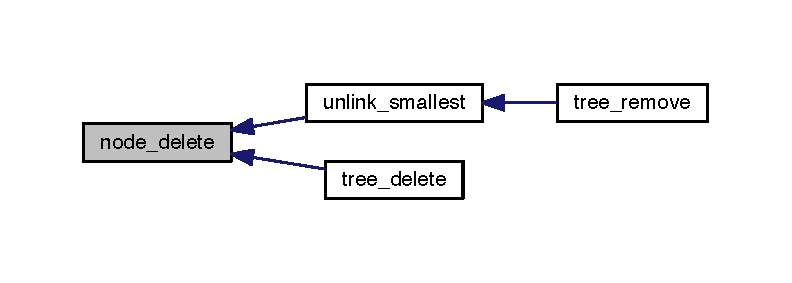
\includegraphics[width=350pt]{node_8c_ae1d068c29b1634d5d867c9837fc666d5_icgraph}
\end{center}
\end{figure}


\hypertarget{node_8c_a9b008ff5bff9290e7d12f61ee6fe0306}{\index{node.\+c@{node.\+c}!node\+\_\+insert@{node\+\_\+insert}}
\index{node\+\_\+insert@{node\+\_\+insert}!node.\+c@{node.\+c}}
\subsubsection[{node\+\_\+insert}]{\setlength{\rightskip}{0pt plus 5cm}void node\+\_\+insert (
\begin{DoxyParamCaption}
\item[{{\bf cmp\+\_\+f}}]{key\+\_\+cmp, }
\item[{void $\ast$}]{k, }
\item[{void $\ast$}]{v, }
\item[{{\bf node\+\_\+s} $\ast$$\ast$}]{n, }
\item[{bool}]{balance}
\end{DoxyParamCaption}
)}}\label{node_8c_a9b008ff5bff9290e7d12f61ee6fe0306}


Stoppar in ett nytt element i trädet. 



Här är anropnings diagrammet för den här funktionen\+:
\nopagebreak
\begin{figure}[H]
\begin{center}
\leavevmode
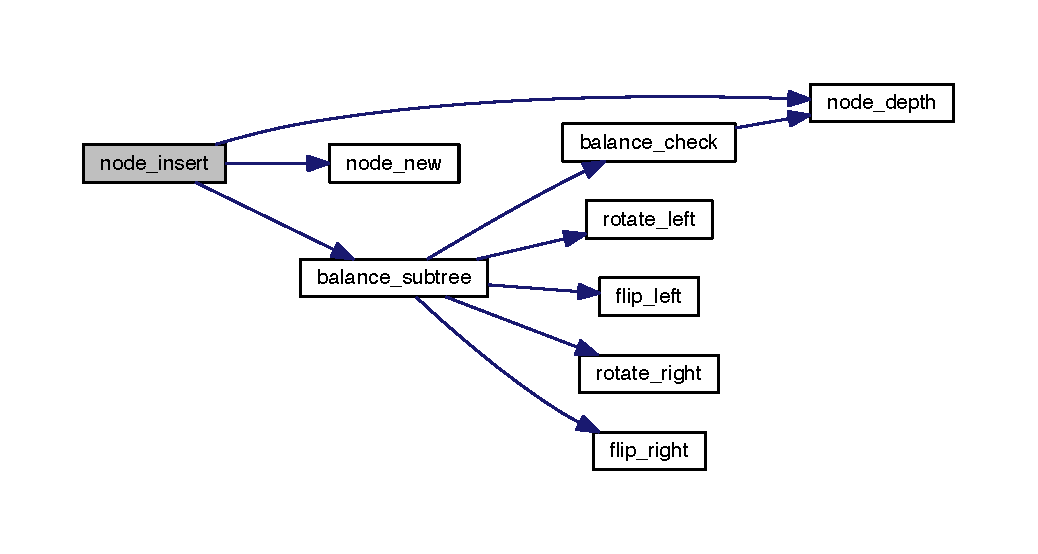
\includegraphics[width=350pt]{node_8c_a9b008ff5bff9290e7d12f61ee6fe0306_cgraph}
\end{center}
\end{figure}




Här är katalog-\/grafen för denna funktion\+:
\nopagebreak
\begin{figure}[H]
\begin{center}
\leavevmode
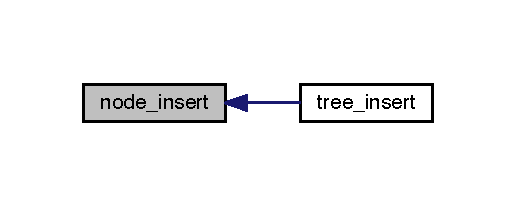
\includegraphics[width=248pt]{node_8c_a9b008ff5bff9290e7d12f61ee6fe0306_icgraph}
\end{center}
\end{figure}


\hypertarget{node_8c_a51b804eb853b5938a60dbe0df42b474a}{\index{node.\+c@{node.\+c}!node\+\_\+new@{node\+\_\+new}}
\index{node\+\_\+new@{node\+\_\+new}!node.\+c@{node.\+c}}
\subsubsection[{node\+\_\+new}]{\setlength{\rightskip}{0pt plus 5cm}{\bf node\+\_\+s}$\ast$ node\+\_\+new (
\begin{DoxyParamCaption}
\item[{void $\ast$}]{k, }
\item[{void $\ast$}]{v}
\end{DoxyParamCaption}
)}}\label{node_8c_a51b804eb853b5938a60dbe0df42b474a}
Skapar en ny nod.


\begin{DoxyParams}{Parametrar}
{\em el} & elementet \\
\hline
\end{DoxyParams}
\begin{DoxyReturn}{Returnerar}
en pekare till en ny nod som allokerats på heapen 
\end{DoxyReturn}


Här är katalog-\/grafen för denna funktion\+:
\nopagebreak
\begin{figure}[H]
\begin{center}
\leavevmode
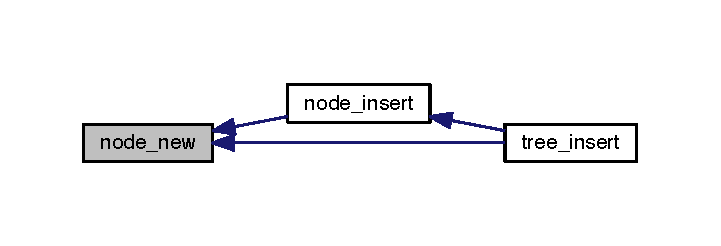
\includegraphics[width=346pt]{node_8c_a51b804eb853b5938a60dbe0df42b474a_icgraph}
\end{center}
\end{figure}


\hypertarget{node_8c_a54482a8cdcd1d716d098fb8e759e5a56}{\index{node.\+c@{node.\+c}!node\+\_\+traversal@{node\+\_\+traversal}}
\index{node\+\_\+traversal@{node\+\_\+traversal}!node.\+c@{node.\+c}}
\subsubsection[{node\+\_\+traversal}]{\setlength{\rightskip}{0pt plus 5cm}void node\+\_\+traversal (
\begin{DoxyParamCaption}
\item[{enum {\bf order}}]{order, }
\item[{{\bf node\+\_\+s} $\ast$}]{n, }
\item[{{\bf apply\+\_\+f}}]{f, }
\item[{void $\ast$}]{arg, }
\item[{bool}]{called\+\_\+internally}
\end{DoxyParamCaption}
)}}\label{node_8c_a54482a8cdcd1d716d098fb8e759e5a56}


Traverserar subträdet. 

\begin{DoxySeeAlso}{Se även}
\hyperlink{tree_8h_adc1ae204ca89e92d85d8b05878708e72}{tree\+\_\+traversal} 
\end{DoxySeeAlso}


Här är anropnings diagrammet för den här funktionen\+:
\nopagebreak
\begin{figure}[H]
\begin{center}
\leavevmode
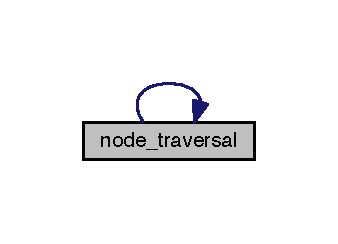
\includegraphics[width=162pt]{node_8c_a54482a8cdcd1d716d098fb8e759e5a56_cgraph}
\end{center}
\end{figure}




Här är katalog-\/grafen för denna funktion\+:
\nopagebreak
\begin{figure}[H]
\begin{center}
\leavevmode
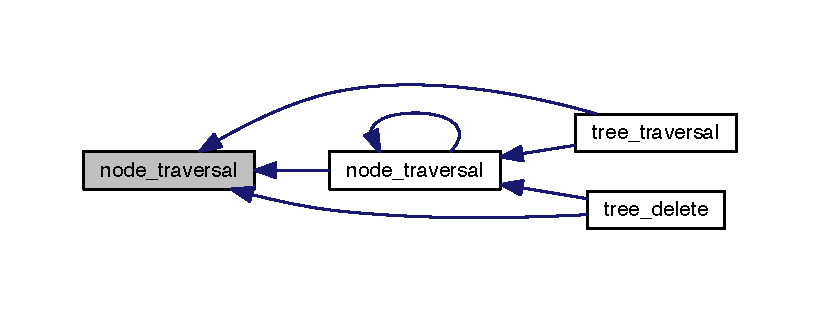
\includegraphics[width=350pt]{node_8c_a54482a8cdcd1d716d098fb8e759e5a56_icgraph}
\end{center}
\end{figure}


\hypertarget{node_8c_a2d121428f77a50dbda46a08eeec930fd}{\index{node.\+c@{node.\+c}!unlink\+\_\+smallest@{unlink\+\_\+smallest}}
\index{unlink\+\_\+smallest@{unlink\+\_\+smallest}!node.\+c@{node.\+c}}
\subsubsection[{unlink\+\_\+smallest}]{\setlength{\rightskip}{0pt plus 5cm}struct {\bf key\+\_\+value} unlink\+\_\+smallest (
\begin{DoxyParamCaption}
\item[{{\bf node\+\_\+s} $\ast$$\ast$}]{n\+\_\+field}
\end{DoxyParamCaption}
)}}\label{node_8c_a2d121428f77a50dbda46a08eeec930fd}
Tar bort den minsta lövnoden i trädet och returnerar en pekare till dess element. 
\begin{DoxyParams}{Parametrar}
{\em n\+\_\+field} & en pekare till föräldranodens höger/vänster-\/post \\
\hline
\end{DoxyParams}


Här är anropnings diagrammet för den här funktionen\+:
\nopagebreak
\begin{figure}[H]
\begin{center}
\leavevmode
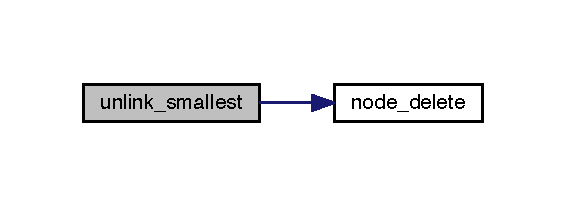
\includegraphics[width=271pt]{node_8c_a2d121428f77a50dbda46a08eeec930fd_cgraph}
\end{center}
\end{figure}




Här är katalog-\/grafen för denna funktion\+:
\nopagebreak
\begin{figure}[H]
\begin{center}
\leavevmode
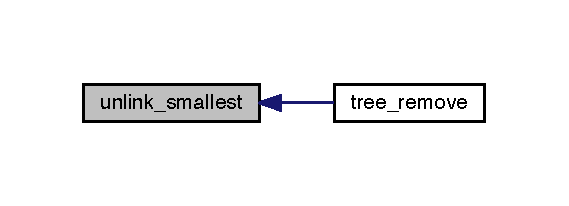
\includegraphics[width=273pt]{node_8c_a2d121428f77a50dbda46a08eeec930fd_icgraph}
\end{center}
\end{figure}



\hypertarget{node_8h}{\section{tree/node.h filreferens}
\label{node_8h}\index{tree/node.\+h@{tree/node.\+h}}
}
{\ttfamily \#include $<$stdbool.\+h$>$}\\*
{\ttfamily \#include $<$stdint.\+h$>$}\\*
{\ttfamily \#include \char`\"{}tree.\+h\char`\"{}}\\*
Include-\/beroendediagram för node.\+h\+:
\nopagebreak
\begin{figure}[H]
\begin{center}
\leavevmode
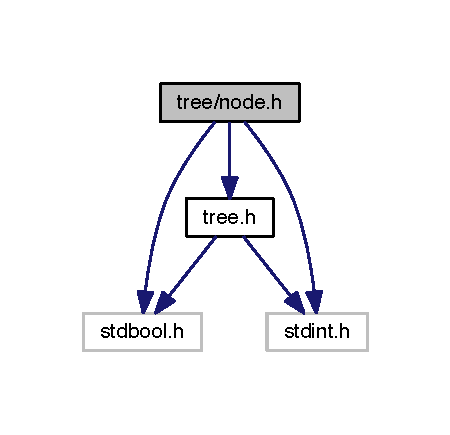
\includegraphics[width=216pt]{node_8h__incl}
\end{center}
\end{figure}
Den här grafen visar vilka filer som direkt eller indirekt inkluderar denna filen.
\nopagebreak
\begin{figure}[H]
\begin{center}
\leavevmode
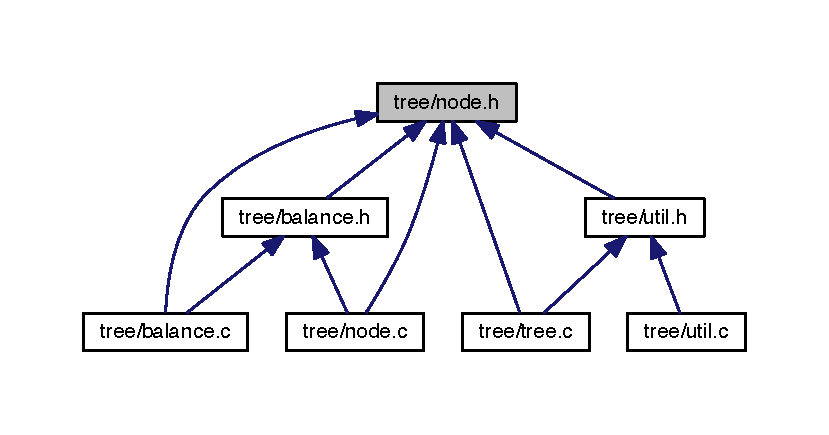
\includegraphics[width=350pt]{node_8h__dep__incl}
\end{center}
\end{figure}
\subsection*{Datastrukturer}
\begin{DoxyCompactItemize}
\item 
struct \hyperlink{structnode}{node}
\item 
struct \hyperlink{structkey__value}{key\+\_\+value}
\end{DoxyCompactItemize}
\subsection*{Typdefinitioner}
\begin{DoxyCompactItemize}
\item 
typedef struct \hyperlink{structnode}{node} \hyperlink{node_8h_aeed67813c57d1b99aba54f16aa01639f}{node\+\_\+s}
\end{DoxyCompactItemize}
\subsection*{Funktioner}
\begin{DoxyCompactItemize}
\item 
\hyperlink{node_8h_aeed67813c57d1b99aba54f16aa01639f}{node\+\_\+s} $\ast$ \hyperlink{node_8h_a51b804eb853b5938a60dbe0df42b474a}{node\+\_\+new} (void $\ast$k, void $\ast$v)
\item 
struct \hyperlink{structkey__value}{key\+\_\+value} \hyperlink{node_8h_ae1d068c29b1634d5d867c9837fc666d5}{node\+\_\+delete} (\hyperlink{node_8h_aeed67813c57d1b99aba54f16aa01639f}{node\+\_\+s} $\ast$n)
\begin{DoxyCompactList}\small\item\em Tar bort en nod ur minnet och returnerar en pekare till dess element. \end{DoxyCompactList}\item 
uint32\+\_\+t \hyperlink{node_8h_a3934222d89b56dbe6612d3128f9fe4da}{node\+\_\+depth} (\hyperlink{node_8h_aeed67813c57d1b99aba54f16aa01639f}{node\+\_\+s} $\ast$n)
\begin{DoxyCompactList}\small\item\em Returnerar subträdets djup. \end{DoxyCompactList}\item 
uint32\+\_\+t \hyperlink{node_8h_ac334fa878f7aa93d140875390c4eed10}{node\+\_\+size} (\hyperlink{node_8h_aeed67813c57d1b99aba54f16aa01639f}{node\+\_\+s} $\ast$n)
\begin{DoxyCompactList}\small\item\em Returnerar subträdets storlek. \end{DoxyCompactList}\item 
void \hyperlink{node_8h_ad40e3b1a3cd655828be0bee052f954ba}{node\+\_\+traversal} (enum \hyperlink{tree_8h_a9f4e8630516f3da89537313b4c828759}{order} \hyperlink{tree_8h_a9f4e8630516f3da89537313b4c828759}{order}, \hyperlink{node_8h_aeed67813c57d1b99aba54f16aa01639f}{node\+\_\+s} $\ast$n, \hyperlink{tree_8h_a9e54f1284e25a3766511292f740cfdf6}{apply\+\_\+f} f, void $\ast$arg, bool called\+\_\+internally)
\begin{DoxyCompactList}\small\item\em Traverserar subträdet. \end{DoxyCompactList}\item 
struct \hyperlink{structkey__value}{key\+\_\+value} \hyperlink{node_8h_a63c4186aa2465e7b9e994de8f570808f}{unlink\+\_\+smallest} (\hyperlink{node_8h_aeed67813c57d1b99aba54f16aa01639f}{node\+\_\+s} $\ast$$\ast$n\+\_\+field)
\item 
void \hyperlink{node_8h_a9b008ff5bff9290e7d12f61ee6fe0306}{node\+\_\+insert} (\hyperlink{tree_8h_ac9404bce0090a72ec95c26c1fc58e4dd}{cmp\+\_\+f} key\+\_\+cmp, void $\ast$k, void $\ast$v, \hyperlink{node_8h_aeed67813c57d1b99aba54f16aa01639f}{node\+\_\+s} $\ast$$\ast$n, bool \hyperlink{balance_8c_a1e7ef09ce66d09456a55c47a8c42f3dc}{balance})
\begin{DoxyCompactList}\small\item\em Stoppar in ett nytt element i trädet. \end{DoxyCompactList}\end{DoxyCompactItemize}


\subsection{Dokumentation över typdefinitioner}
\hypertarget{node_8h_aeed67813c57d1b99aba54f16aa01639f}{\index{node.\+h@{node.\+h}!node\+\_\+s@{node\+\_\+s}}
\index{node\+\_\+s@{node\+\_\+s}!node.\+h@{node.\+h}}
\subsubsection[{node\+\_\+s}]{\setlength{\rightskip}{0pt plus 5cm}typedef struct {\bf node} {\bf node\+\_\+s}}}\label{node_8h_aeed67813c57d1b99aba54f16aa01639f}


\subsection{Dokumentation över funktioner}
\hypertarget{node_8h_ae1d068c29b1634d5d867c9837fc666d5}{\index{node.\+h@{node.\+h}!node\+\_\+delete@{node\+\_\+delete}}
\index{node\+\_\+delete@{node\+\_\+delete}!node.\+h@{node.\+h}}
\subsubsection[{node\+\_\+delete}]{\setlength{\rightskip}{0pt plus 5cm}struct {\bf key\+\_\+value} node\+\_\+delete (
\begin{DoxyParamCaption}
\item[{{\bf node\+\_\+s} $\ast$}]{n}
\end{DoxyParamCaption}
)}}\label{node_8h_ae1d068c29b1634d5d867c9837fc666d5}


Tar bort en nod ur minnet och returnerar en pekare till dess element. 



Här är katalog-\/grafen för denna funktion\+:
\nopagebreak
\begin{figure}[H]
\begin{center}
\leavevmode
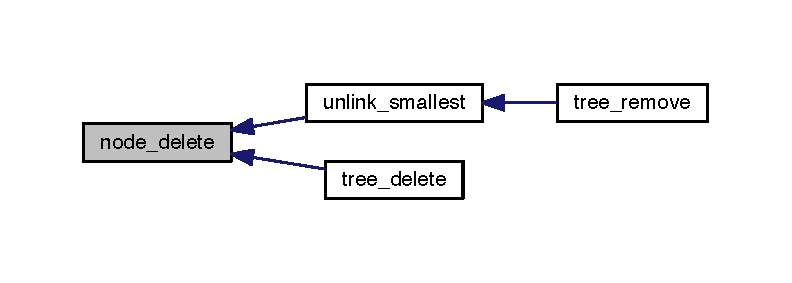
\includegraphics[width=350pt]{node_8h_ae1d068c29b1634d5d867c9837fc666d5_icgraph}
\end{center}
\end{figure}


\hypertarget{node_8h_a3934222d89b56dbe6612d3128f9fe4da}{\index{node.\+h@{node.\+h}!node\+\_\+depth@{node\+\_\+depth}}
\index{node\+\_\+depth@{node\+\_\+depth}!node.\+h@{node.\+h}}
\subsubsection[{node\+\_\+depth}]{\setlength{\rightskip}{0pt plus 5cm}uint32\+\_\+t node\+\_\+depth (
\begin{DoxyParamCaption}
\item[{{\bf node\+\_\+s} $\ast$}]{n}
\end{DoxyParamCaption}
)}}\label{node_8h_a3934222d89b56dbe6612d3128f9fe4da}


Returnerar subträdets djup. 

\begin{DoxySeeAlso}{Se även}
\hyperlink{tree_8h_a41f3b7564a5da77967a40e2f484e73a8}{tree\+\_\+depth} 
\end{DoxySeeAlso}


Här är katalog-\/grafen för denna funktion\+:
\nopagebreak
\begin{figure}[H]
\begin{center}
\leavevmode
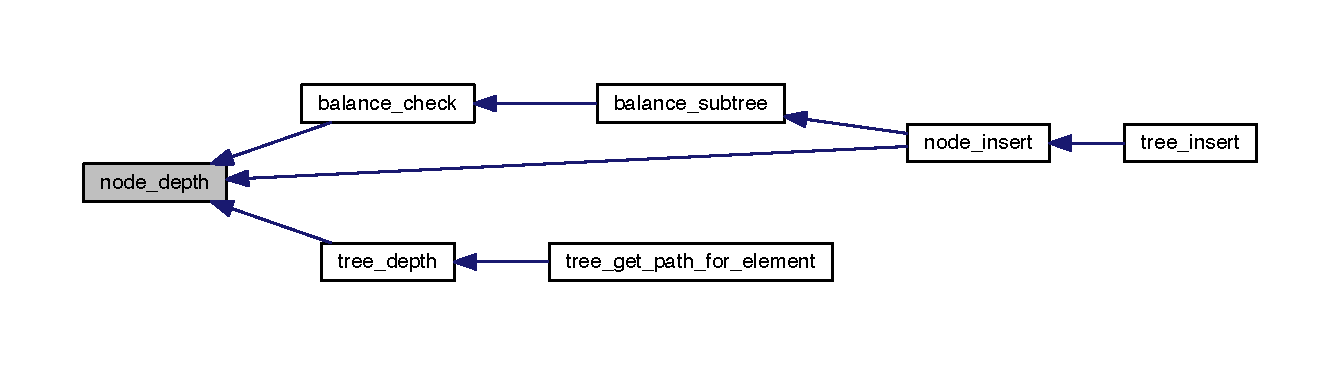
\includegraphics[width=350pt]{node_8h_a3934222d89b56dbe6612d3128f9fe4da_icgraph}
\end{center}
\end{figure}


\hypertarget{node_8h_a9b008ff5bff9290e7d12f61ee6fe0306}{\index{node.\+h@{node.\+h}!node\+\_\+insert@{node\+\_\+insert}}
\index{node\+\_\+insert@{node\+\_\+insert}!node.\+h@{node.\+h}}
\subsubsection[{node\+\_\+insert}]{\setlength{\rightskip}{0pt plus 5cm}void node\+\_\+insert (
\begin{DoxyParamCaption}
\item[{{\bf cmp\+\_\+f}}]{key\+\_\+cmp, }
\item[{void $\ast$}]{k, }
\item[{void $\ast$}]{v, }
\item[{{\bf node\+\_\+s} $\ast$$\ast$}]{n, }
\item[{bool}]{balance}
\end{DoxyParamCaption}
)}}\label{node_8h_a9b008ff5bff9290e7d12f61ee6fe0306}


Stoppar in ett nytt element i trädet. 



Här är anropnings diagrammet för den här funktionen\+:
\nopagebreak
\begin{figure}[H]
\begin{center}
\leavevmode
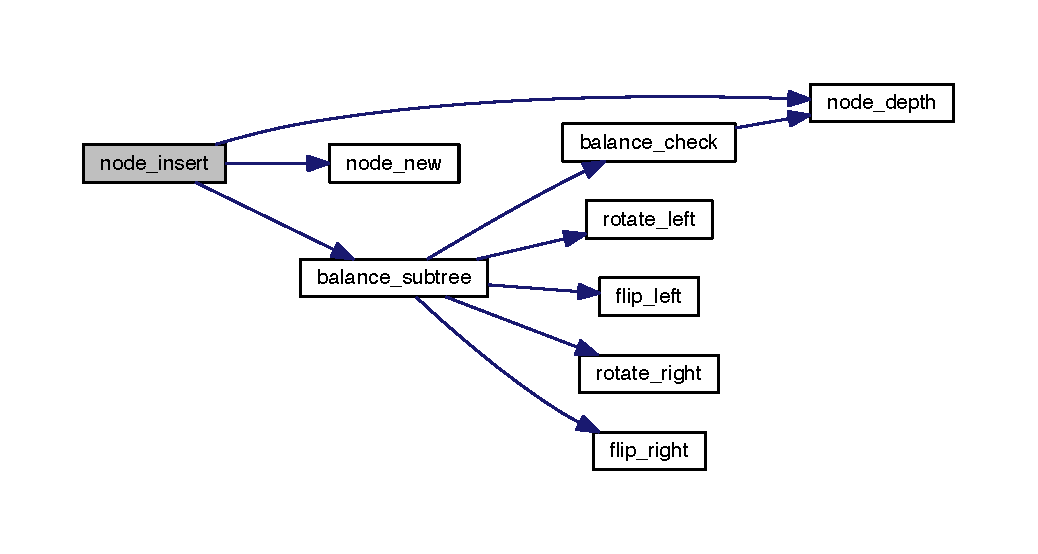
\includegraphics[width=350pt]{node_8h_a9b008ff5bff9290e7d12f61ee6fe0306_cgraph}
\end{center}
\end{figure}




Här är katalog-\/grafen för denna funktion\+:
\nopagebreak
\begin{figure}[H]
\begin{center}
\leavevmode
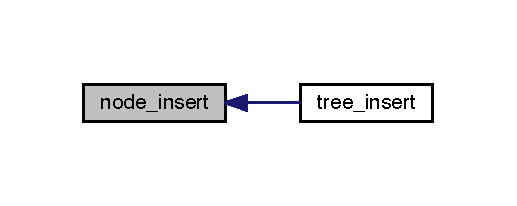
\includegraphics[width=248pt]{node_8h_a9b008ff5bff9290e7d12f61ee6fe0306_icgraph}
\end{center}
\end{figure}


\hypertarget{node_8h_a51b804eb853b5938a60dbe0df42b474a}{\index{node.\+h@{node.\+h}!node\+\_\+new@{node\+\_\+new}}
\index{node\+\_\+new@{node\+\_\+new}!node.\+h@{node.\+h}}
\subsubsection[{node\+\_\+new}]{\setlength{\rightskip}{0pt plus 5cm}{\bf node\+\_\+s}$\ast$ node\+\_\+new (
\begin{DoxyParamCaption}
\item[{void $\ast$}]{k, }
\item[{void $\ast$}]{v}
\end{DoxyParamCaption}
)}}\label{node_8h_a51b804eb853b5938a60dbe0df42b474a}
Skapar en ny nod.


\begin{DoxyParams}{Parametrar}
{\em el} & elementet \\
\hline
\end{DoxyParams}
\begin{DoxyReturn}{Returnerar}
en pekare till en ny nod som allokerats på heapen 
\end{DoxyReturn}


Här är katalog-\/grafen för denna funktion\+:
\nopagebreak
\begin{figure}[H]
\begin{center}
\leavevmode
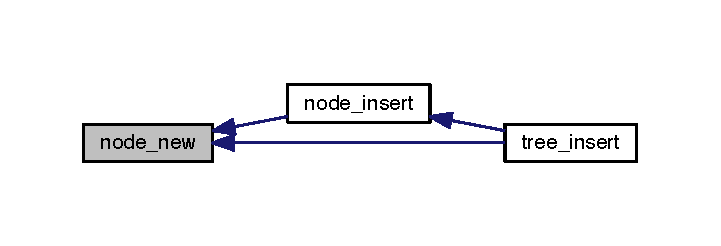
\includegraphics[width=346pt]{node_8h_a51b804eb853b5938a60dbe0df42b474a_icgraph}
\end{center}
\end{figure}


\hypertarget{node_8h_ac334fa878f7aa93d140875390c4eed10}{\index{node.\+h@{node.\+h}!node\+\_\+size@{node\+\_\+size}}
\index{node\+\_\+size@{node\+\_\+size}!node.\+h@{node.\+h}}
\subsubsection[{node\+\_\+size}]{\setlength{\rightskip}{0pt plus 5cm}uint32\+\_\+t node\+\_\+size (
\begin{DoxyParamCaption}
\item[{{\bf node\+\_\+s} $\ast$}]{n}
\end{DoxyParamCaption}
)}}\label{node_8h_ac334fa878f7aa93d140875390c4eed10}


Returnerar subträdets storlek. 

\begin{DoxySeeAlso}{Se även}
\hyperlink{tree_8h_a1c9d41a0f10a772536b25cbf7b992c7a}{tree\+\_\+size} 
\end{DoxySeeAlso}


Här är katalog-\/grafen för denna funktion\+:
\nopagebreak
\begin{figure}[H]
\begin{center}
\leavevmode
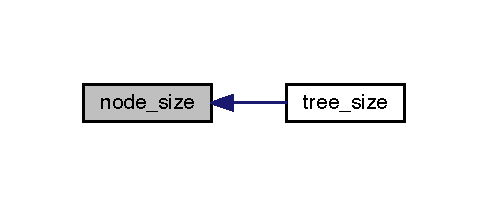
\includegraphics[width=234pt]{node_8h_ac334fa878f7aa93d140875390c4eed10_icgraph}
\end{center}
\end{figure}


\hypertarget{node_8h_ad40e3b1a3cd655828be0bee052f954ba}{\index{node.\+h@{node.\+h}!node\+\_\+traversal@{node\+\_\+traversal}}
\index{node\+\_\+traversal@{node\+\_\+traversal}!node.\+h@{node.\+h}}
\subsubsection[{node\+\_\+traversal}]{\setlength{\rightskip}{0pt plus 5cm}void node\+\_\+traversal (
\begin{DoxyParamCaption}
\item[{enum {\bf order}}]{order, }
\item[{{\bf node\+\_\+s} $\ast$}]{n, }
\item[{{\bf apply\+\_\+f}}]{f, }
\item[{void $\ast$}]{arg, }
\item[{bool}]{called\+\_\+internally}
\end{DoxyParamCaption}
)}}\label{node_8h_ad40e3b1a3cd655828be0bee052f954ba}


Traverserar subträdet. 

\begin{DoxySeeAlso}{Se även}
\hyperlink{tree_8h_adc1ae204ca89e92d85d8b05878708e72}{tree\+\_\+traversal} 
\end{DoxySeeAlso}


Här är anropnings diagrammet för den här funktionen\+:
\nopagebreak
\begin{figure}[H]
\begin{center}
\leavevmode
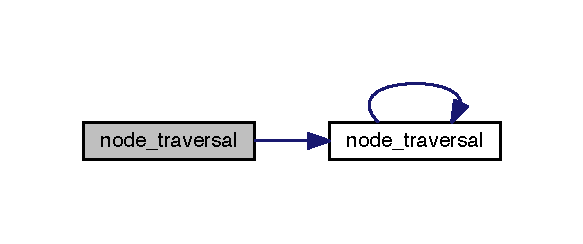
\includegraphics[width=280pt]{node_8h_ad40e3b1a3cd655828be0bee052f954ba_cgraph}
\end{center}
\end{figure}




Här är katalog-\/grafen för denna funktion\+:
\nopagebreak
\begin{figure}[H]
\begin{center}
\leavevmode
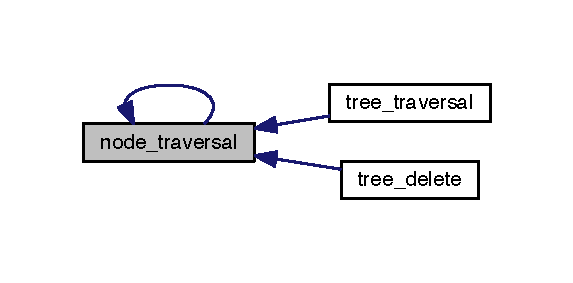
\includegraphics[width=275pt]{node_8h_ad40e3b1a3cd655828be0bee052f954ba_icgraph}
\end{center}
\end{figure}


\hypertarget{node_8h_a63c4186aa2465e7b9e994de8f570808f}{\index{node.\+h@{node.\+h}!unlink\+\_\+smallest@{unlink\+\_\+smallest}}
\index{unlink\+\_\+smallest@{unlink\+\_\+smallest}!node.\+h@{node.\+h}}
\subsubsection[{unlink\+\_\+smallest}]{\setlength{\rightskip}{0pt plus 5cm}struct {\bf key\+\_\+value} unlink\+\_\+smallest (
\begin{DoxyParamCaption}
\item[{{\bf node\+\_\+s} $\ast$$\ast$}]{n\+\_\+field}
\end{DoxyParamCaption}
)}}\label{node_8h_a63c4186aa2465e7b9e994de8f570808f}
Tar bort den minsta lövnoden i trädet och returnerar en pekare till dess element. 
\begin{DoxyParams}{Parametrar}
{\em n\+\_\+field} & en pekare till föräldranodens höger/vänster-\/post \\
\hline
\end{DoxyParams}


Här är anropnings diagrammet för den här funktionen\+:
\nopagebreak
\begin{figure}[H]
\begin{center}
\leavevmode
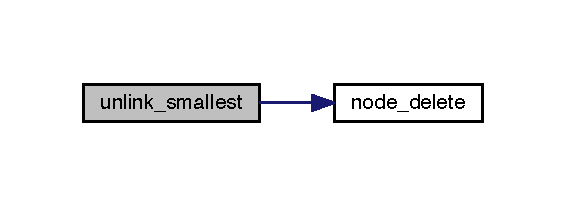
\includegraphics[width=271pt]{node_8h_a63c4186aa2465e7b9e994de8f570808f_cgraph}
\end{center}
\end{figure}




Här är katalog-\/grafen för denna funktion\+:
\nopagebreak
\begin{figure}[H]
\begin{center}
\leavevmode
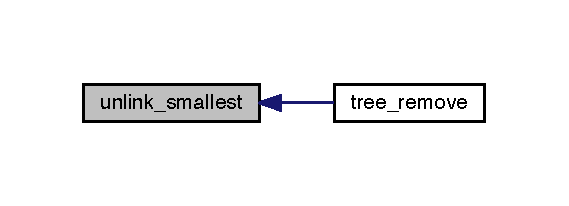
\includegraphics[width=273pt]{node_8h_a63c4186aa2465e7b9e994de8f570808f_icgraph}
\end{center}
\end{figure}



\hypertarget{tree_8c}{\section{tree/tree.c filreferens}
\label{tree_8c}\index{tree/tree.\+c@{tree/tree.\+c}}
}
{\ttfamily \#include $<$stdlib.\+h$>$}\\*
{\ttfamily \#include $<$assert.\+h$>$}\\*
{\ttfamily \#include \char`\"{}tree.\+h\char`\"{}}\\*
{\ttfamily \#include \char`\"{}node.\+h\char`\"{}}\\*
{\ttfamily \#include \char`\"{}util.\+h\char`\"{}}\\*
Include-\/beroendediagram för tree.\+c\+:
\nopagebreak
\begin{figure}[H]
\begin{center}
\leavevmode
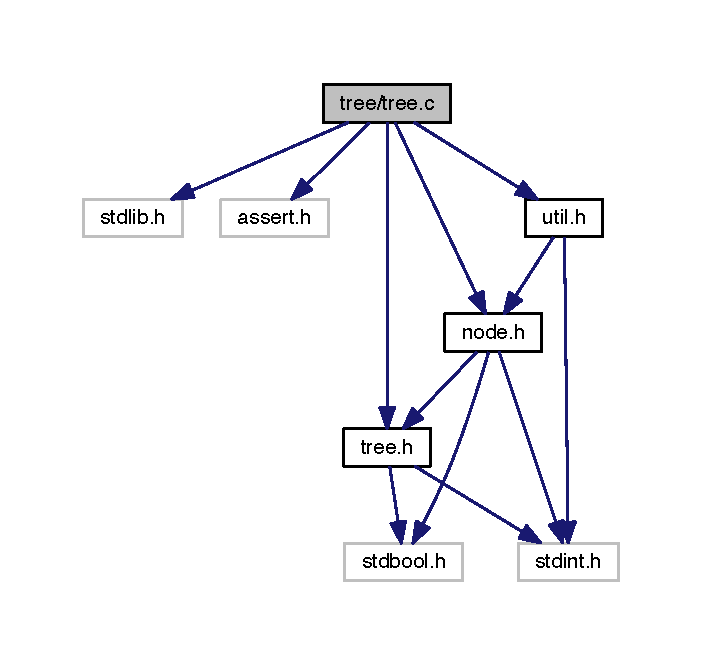
\includegraphics[width=337pt]{tree_8c__incl}
\end{center}
\end{figure}
\subsection*{Datastrukturer}
\begin{DoxyCompactItemize}
\item 
struct \hyperlink{structtree}{tree}
\end{DoxyCompactItemize}
\subsection*{Definitioner}
\begin{DoxyCompactItemize}
\item 
\#define \hyperlink{tree_8c_aace936c30e3b97b67d64c80c2e7dbc4c}{No\+\_\+left\+\_\+subtree}(n)~((n)-\/$>$left == N\+U\+L\+L)
\item 
\#define \hyperlink{tree_8c_ab0a57256803646ba09d50c898cefb82b}{No\+\_\+right\+\_\+subtree}(n)~((n)-\/$>$right == N\+U\+L\+L)
\item 
\#define \hyperlink{tree_8c_a71ce371d9c132b3e5b9e389fc18fcbce}{Is\+\_\+leaf}(n)~(\hyperlink{tree_8c_ab0a57256803646ba09d50c898cefb82b}{No\+\_\+right\+\_\+subtree}(n) \&\& \hyperlink{tree_8c_aace936c30e3b97b67d64c80c2e7dbc4c}{No\+\_\+left\+\_\+subtree}(n))
\end{DoxyCompactItemize}
\subsection*{Funktioner}
\begin{DoxyCompactItemize}
\item 
void $\ast$ \hyperlink{tree_8c_ae7f8766a04f543e0208390c5a8981c27}{tree\+\_\+get} (\hyperlink{tree_8h_a563df572fa7aabc17e5f9981cd99460b}{tree\+\_\+s} $\ast$t, void $\ast$k)
\item 
void \hyperlink{tree_8c_a5d8936e5b6a90176fd35f7999a1820b8}{tree\+\_\+traversal} (enum \hyperlink{tree_8h_a9f4e8630516f3da89537313b4c828759}{order} \hyperlink{tree_8h_a9f4e8630516f3da89537313b4c828759}{order}, \hyperlink{tree_8h_a563df572fa7aabc17e5f9981cd99460b}{tree\+\_\+s} $\ast$t, \hyperlink{tree_8h_a9e54f1284e25a3766511292f740cfdf6}{apply\+\_\+f} f, void $\ast$fst\+\_\+arg)
\item 
\hyperlink{tree_8h_a563df572fa7aabc17e5f9981cd99460b}{tree\+\_\+s} $\ast$ \hyperlink{tree_8c_a3797e9d77dd03723b9f79708b93ba3bf}{tree\+\_\+new} (\hyperlink{tree_8h_ac9404bce0090a72ec95c26c1fc58e4dd}{cmp\+\_\+f} f, bool b)
\item 
void \hyperlink{tree_8c_a6f1cdce17a27cbc4d82e48656190ffe3}{tree\+\_\+delete} (\hyperlink{tree_8h_a563df572fa7aabc17e5f9981cd99460b}{tree\+\_\+s} $\ast$t)
\item 
void \hyperlink{tree_8c_a4d042ef97247fae341fc3205a5cdec79}{tree\+\_\+insert} (\hyperlink{tree_8h_a563df572fa7aabc17e5f9981cd99460b}{tree\+\_\+s} $\ast$t, void $\ast$k, void $\ast$v)
\item 
void $\ast$ \hyperlink{tree_8c_a31c4190c6bb6612b52790ca73ceee500}{tree\+\_\+remove} (\hyperlink{tree_8h_a563df572fa7aabc17e5f9981cd99460b}{tree\+\_\+s} $\ast$t, void $\ast$k)
\item 
void $\ast$ \hyperlink{tree_8c_a6d1dc22883d9d3d466cf0e917ad793af}{tree\+\_\+get\+\_\+element\+\_\+for\+\_\+path} (\hyperlink{tree_8h_a563df572fa7aabc17e5f9981cd99460b}{tree\+\_\+s} $\ast$t, char $\ast$path)
\item 
char $\ast$ \hyperlink{tree_8c_ac94f77e669d14b11052ba0fcf2339371}{tree\+\_\+get\+\_\+path\+\_\+for\+\_\+element} (\hyperlink{tree_8h_a563df572fa7aabc17e5f9981cd99460b}{tree\+\_\+s} $\ast$t, void $\ast$k)
\item 
uint32\+\_\+t \hyperlink{tree_8c_aaab29a3b7476b666ac81872398b2a91e}{tree\+\_\+depth} (\hyperlink{tree_8h_a563df572fa7aabc17e5f9981cd99460b}{tree\+\_\+s} $\ast$t)
\item 
uint32\+\_\+t \hyperlink{tree_8c_abbd772c62da9bafb66ac5513ee870735}{tree\+\_\+size} (\hyperlink{tree_8h_a563df572fa7aabc17e5f9981cd99460b}{tree\+\_\+s} $\ast$t)
\end{DoxyCompactItemize}


\subsection{Dokumentation över definitioner}
\hypertarget{tree_8c_a71ce371d9c132b3e5b9e389fc18fcbce}{\index{tree.\+c@{tree.\+c}!Is\+\_\+leaf@{Is\+\_\+leaf}}
\index{Is\+\_\+leaf@{Is\+\_\+leaf}!tree.\+c@{tree.\+c}}
\subsubsection[{Is\+\_\+leaf}]{\setlength{\rightskip}{0pt plus 5cm}\#define Is\+\_\+leaf(
\begin{DoxyParamCaption}
\item[{}]{n}
\end{DoxyParamCaption}
)~({\bf No\+\_\+right\+\_\+subtree}(n) \&\& {\bf No\+\_\+left\+\_\+subtree}(n))}}\label{tree_8c_a71ce371d9c132b3e5b9e389fc18fcbce}
\hypertarget{tree_8c_aace936c30e3b97b67d64c80c2e7dbc4c}{\index{tree.\+c@{tree.\+c}!No\+\_\+left\+\_\+subtree@{No\+\_\+left\+\_\+subtree}}
\index{No\+\_\+left\+\_\+subtree@{No\+\_\+left\+\_\+subtree}!tree.\+c@{tree.\+c}}
\subsubsection[{No\+\_\+left\+\_\+subtree}]{\setlength{\rightskip}{0pt plus 5cm}\#define No\+\_\+left\+\_\+subtree(
\begin{DoxyParamCaption}
\item[{}]{n}
\end{DoxyParamCaption}
)~((n)-\/$>$left == N\+U\+L\+L)}}\label{tree_8c_aace936c30e3b97b67d64c80c2e7dbc4c}
\hypertarget{tree_8c_ab0a57256803646ba09d50c898cefb82b}{\index{tree.\+c@{tree.\+c}!No\+\_\+right\+\_\+subtree@{No\+\_\+right\+\_\+subtree}}
\index{No\+\_\+right\+\_\+subtree@{No\+\_\+right\+\_\+subtree}!tree.\+c@{tree.\+c}}
\subsubsection[{No\+\_\+right\+\_\+subtree}]{\setlength{\rightskip}{0pt plus 5cm}\#define No\+\_\+right\+\_\+subtree(
\begin{DoxyParamCaption}
\item[{}]{n}
\end{DoxyParamCaption}
)~((n)-\/$>$right == N\+U\+L\+L)}}\label{tree_8c_ab0a57256803646ba09d50c898cefb82b}


\subsection{Dokumentation över funktioner}
\hypertarget{tree_8c_a6f1cdce17a27cbc4d82e48656190ffe3}{\index{tree.\+c@{tree.\+c}!tree\+\_\+delete@{tree\+\_\+delete}}
\index{tree\+\_\+delete@{tree\+\_\+delete}!tree.\+c@{tree.\+c}}
\subsubsection[{tree\+\_\+delete}]{\setlength{\rightskip}{0pt plus 5cm}void tree\+\_\+delete (
\begin{DoxyParamCaption}
\item[{{\bf tree\+\_\+s} $\ast$}]{tree}
\end{DoxyParamCaption}
)}}\label{tree_8c_a6f1cdce17a27cbc4d82e48656190ffe3}
Ta bort trädet ur minnes.


\begin{DoxyParams}{Parametrar}
{\em tree} & trädet\\
\hline
\end{DoxyParams}
Sorteringsnycklar och element tas inte bort ur minnet. 

Här är anropnings diagrammet för den här funktionen\+:
\nopagebreak
\begin{figure}[H]
\begin{center}
\leavevmode
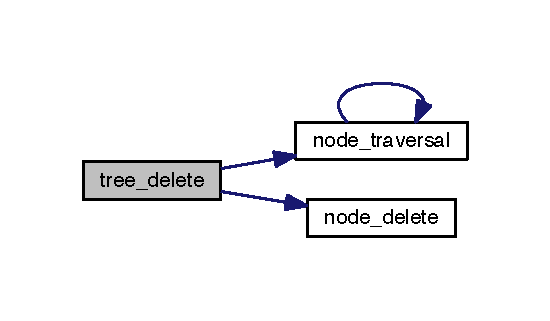
\includegraphics[width=264pt]{tree_8c_a6f1cdce17a27cbc4d82e48656190ffe3_cgraph}
\end{center}
\end{figure}


\hypertarget{tree_8c_aaab29a3b7476b666ac81872398b2a91e}{\index{tree.\+c@{tree.\+c}!tree\+\_\+depth@{tree\+\_\+depth}}
\index{tree\+\_\+depth@{tree\+\_\+depth}!tree.\+c@{tree.\+c}}
\subsubsection[{tree\+\_\+depth}]{\setlength{\rightskip}{0pt plus 5cm}uint32\+\_\+t tree\+\_\+depth (
\begin{DoxyParamCaption}
\item[{{\bf tree\+\_\+s} $\ast$}]{tree}
\end{DoxyParamCaption}
)}}\label{tree_8c_aaab29a3b7476b666ac81872398b2a91e}
Returnerar djupet i trädet.


\begin{DoxyParams}{Parametrar}
{\em tree} & trädet \\
\hline
\end{DoxyParams}
\begin{DoxyReturn}{Returnerar}
tree\+:s djup 
\end{DoxyReturn}


Här är anropnings diagrammet för den här funktionen\+:
\nopagebreak
\begin{figure}[H]
\begin{center}
\leavevmode
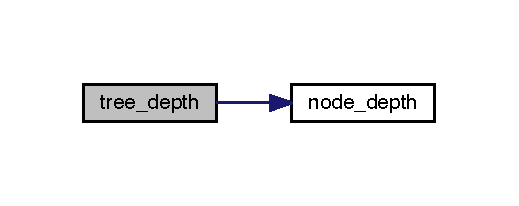
\includegraphics[width=249pt]{tree_8c_aaab29a3b7476b666ac81872398b2a91e_cgraph}
\end{center}
\end{figure}




Här är katalog-\/grafen för denna funktion\+:
\nopagebreak
\begin{figure}[H]
\begin{center}
\leavevmode
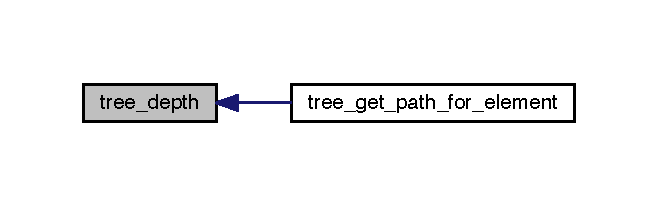
\includegraphics[width=316pt]{tree_8c_aaab29a3b7476b666ac81872398b2a91e_icgraph}
\end{center}
\end{figure}


\hypertarget{tree_8c_ae7f8766a04f543e0208390c5a8981c27}{\index{tree.\+c@{tree.\+c}!tree\+\_\+get@{tree\+\_\+get}}
\index{tree\+\_\+get@{tree\+\_\+get}!tree.\+c@{tree.\+c}}
\subsubsection[{tree\+\_\+get}]{\setlength{\rightskip}{0pt plus 5cm}void$\ast$ tree\+\_\+get (
\begin{DoxyParamCaption}
\item[{{\bf tree\+\_\+s} $\ast$}]{tree, }
\item[{void $\ast$}]{key}
\end{DoxyParamCaption}
)}}\label{tree_8c_ae7f8766a04f543e0208390c5a8981c27}
Returnerar en pekare till ett element i trädet.


\begin{DoxyParams}{Parametrar}
{\em tree} & trädet \\
\hline
{\em key} & sorteringsnyckeln för det sökta elementet \\
\hline
\end{DoxyParams}
\begin{DoxyReturn}{Returnerar}
det matchande elementet från trädet 
\end{DoxyReturn}
\hypertarget{tree_8c_a6d1dc22883d9d3d466cf0e917ad793af}{\index{tree.\+c@{tree.\+c}!tree\+\_\+get\+\_\+element\+\_\+for\+\_\+path@{tree\+\_\+get\+\_\+element\+\_\+for\+\_\+path}}
\index{tree\+\_\+get\+\_\+element\+\_\+for\+\_\+path@{tree\+\_\+get\+\_\+element\+\_\+for\+\_\+path}!tree.\+c@{tree.\+c}}
\subsubsection[{tree\+\_\+get\+\_\+element\+\_\+for\+\_\+path}]{\setlength{\rightskip}{0pt plus 5cm}void$\ast$ tree\+\_\+get\+\_\+element\+\_\+for\+\_\+path (
\begin{DoxyParamCaption}
\item[{{\bf tree\+\_\+s} $\ast$}]{tree, }
\item[{char $\ast$}]{path}
\end{DoxyParamCaption}
)}}\label{tree_8c_a6d1dc22883d9d3d466cf0e917ad793af}
Tar en sträng med samma format som returneras från tree\+\_\+get\+\_\+path\+\_\+for\+\_\+element och returnerar elementet på den platsen i trädet.


\begin{DoxyParams}{Parametrar}
{\em tree} & trädet \\
\hline
{\em path} & pathen till elementet som skall returneras \\
\hline
\end{DoxyParams}
\begin{DoxyReturn}{Returnerar}
en pekare till ett element eller N\+U\+L\+L 
\end{DoxyReturn}
\hypertarget{tree_8c_ac94f77e669d14b11052ba0fcf2339371}{\index{tree.\+c@{tree.\+c}!tree\+\_\+get\+\_\+path\+\_\+for\+\_\+element@{tree\+\_\+get\+\_\+path\+\_\+for\+\_\+element}}
\index{tree\+\_\+get\+\_\+path\+\_\+for\+\_\+element@{tree\+\_\+get\+\_\+path\+\_\+for\+\_\+element}!tree.\+c@{tree.\+c}}
\subsubsection[{tree\+\_\+get\+\_\+path\+\_\+for\+\_\+element}]{\setlength{\rightskip}{0pt plus 5cm}char$\ast$ tree\+\_\+get\+\_\+path\+\_\+for\+\_\+element (
\begin{DoxyParamCaption}
\item[{{\bf tree\+\_\+s} $\ast$}]{tree, }
\item[{void $\ast$}]{key}
\end{DoxyParamCaption}
)}}\label{tree_8c_ac94f77e669d14b11052ba0fcf2339371}
Returnerar en path till ett element i trädet.

En path kan vara t.\+ex. \char`\"{}\char`\"{} för roten, \char`\"{}\+L\+L\char`\"{} för två steg vänster, \char`\"{}\+L\+R\char`\"{} för vänster-\/höger etc.


\begin{DoxyParams}{Parametrar}
{\em tree} & trädet \\
\hline
{\em key} & sorteringsnyckeln för det sökta elementet \\
\hline
\end{DoxyParams}
\begin{DoxyReturn}{Returnerar}
pathen till el, ev N\+U\+L\+L om el inte finns i trädet 
\end{DoxyReturn}


Här är anropnings diagrammet för den här funktionen\+:
\nopagebreak
\begin{figure}[H]
\begin{center}
\leavevmode
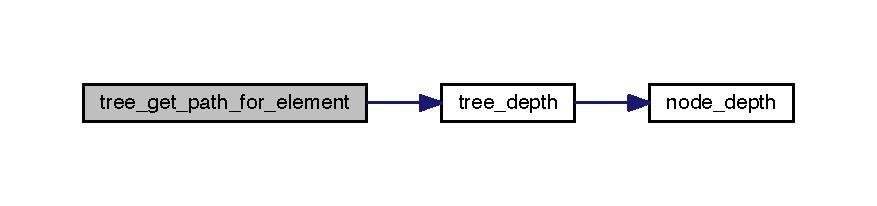
\includegraphics[width=350pt]{tree_8c_ac94f77e669d14b11052ba0fcf2339371_cgraph}
\end{center}
\end{figure}


\hypertarget{tree_8c_a4d042ef97247fae341fc3205a5cdec79}{\index{tree.\+c@{tree.\+c}!tree\+\_\+insert@{tree\+\_\+insert}}
\index{tree\+\_\+insert@{tree\+\_\+insert}!tree.\+c@{tree.\+c}}
\subsubsection[{tree\+\_\+insert}]{\setlength{\rightskip}{0pt plus 5cm}void tree\+\_\+insert (
\begin{DoxyParamCaption}
\item[{{\bf tree\+\_\+s} $\ast$}]{tree, }
\item[{void $\ast$}]{key, }
\item[{void $\ast$}]{value}
\end{DoxyParamCaption}
)}}\label{tree_8c_a4d042ef97247fae341fc3205a5cdec79}
Stoppar in ett element i trädet.

O\+B\+S! Implementationen förutsätter att alla nycklar är unika vid insättning!


\begin{DoxyParams}{Parametrar}
{\em tree} & trädet \\
\hline
{\em key} & sorteringsnyckeln för elementet \\
\hline
{\em value} & elementet som skall stoppas in \\
\hline
\end{DoxyParams}


Här är anropnings diagrammet för den här funktionen\+:
\nopagebreak
\begin{figure}[H]
\begin{center}
\leavevmode
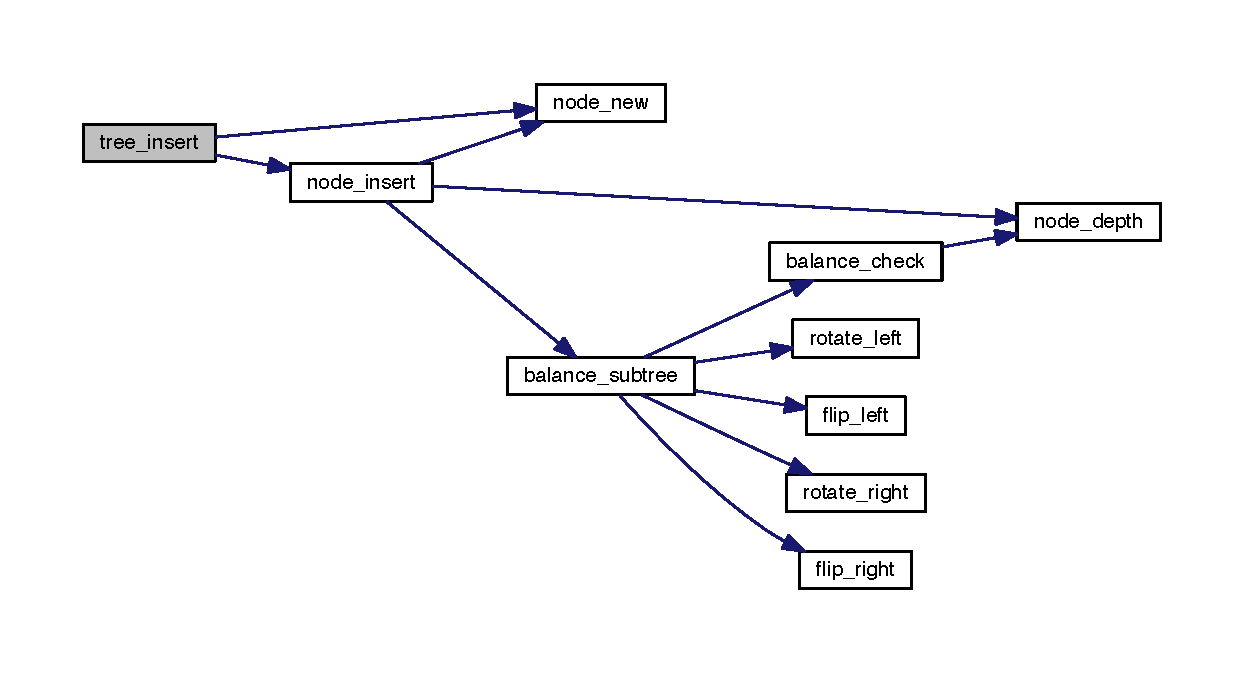
\includegraphics[width=350pt]{tree_8c_a4d042ef97247fae341fc3205a5cdec79_cgraph}
\end{center}
\end{figure}


\hypertarget{tree_8c_a3797e9d77dd03723b9f79708b93ba3bf}{\index{tree.\+c@{tree.\+c}!tree\+\_\+new@{tree\+\_\+new}}
\index{tree\+\_\+new@{tree\+\_\+new}!tree.\+c@{tree.\+c}}
\subsubsection[{tree\+\_\+new}]{\setlength{\rightskip}{0pt plus 5cm}{\bf tree\+\_\+s}$\ast$ tree\+\_\+new (
\begin{DoxyParamCaption}
\item[{{\bf cmp\+\_\+f}}]{key\+\_\+compare\+\_\+function, }
\item[{bool}]{auto\+\_\+balance}
\end{DoxyParamCaption}
)}}\label{tree_8c_a3797e9d77dd03723b9f79708b93ba3bf}
Skapa ett nytt träd.


\begin{DoxyParams}{Parametrar}
{\em key\+\_\+compare\+\_\+function} & pekar ut den jämförelsefunktion som skall användas för att jämföra elementen i trädet \\
\hline
{\em auto\+\_\+balance} & är true om trädet skall balansera sig automatiskt vid insättning och borttagning\\
\hline
\end{DoxyParams}
Jämförelsefunktionen skall fungera som strcmp map returvärden. \hypertarget{tree_8c_a31c4190c6bb6612b52790ca73ceee500}{\index{tree.\+c@{tree.\+c}!tree\+\_\+remove@{tree\+\_\+remove}}
\index{tree\+\_\+remove@{tree\+\_\+remove}!tree.\+c@{tree.\+c}}
\subsubsection[{tree\+\_\+remove}]{\setlength{\rightskip}{0pt plus 5cm}void$\ast$ tree\+\_\+remove (
\begin{DoxyParamCaption}
\item[{{\bf tree\+\_\+s} $\ast$}]{tree, }
\item[{void $\ast$}]{key}
\end{DoxyParamCaption}
)}}\label{tree_8c_a31c4190c6bb6612b52790ca73ceee500}
Tar bort ett element ur trädet.


\begin{DoxyParams}{Parametrar}
{\em tree} & trädet \\
\hline
{\em key} & sorteringsnyckeln för det sökta elementet \\
\hline
\end{DoxyParams}
\begin{DoxyReturn}{Returnerar}
en pekare till elementet eller N\+U\+L\+L om det inte fanns i trädet 
\end{DoxyReturn}


Här är anropnings diagrammet för den här funktionen\+:
\nopagebreak
\begin{figure}[H]
\begin{center}
\leavevmode
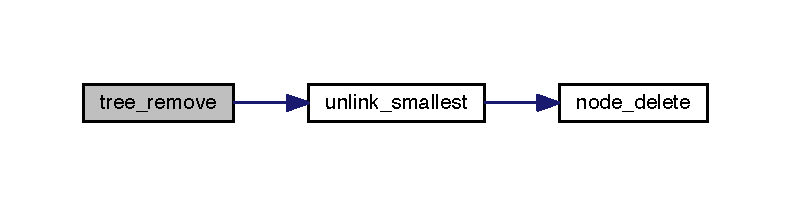
\includegraphics[width=350pt]{tree_8c_a31c4190c6bb6612b52790ca73ceee500_cgraph}
\end{center}
\end{figure}


\hypertarget{tree_8c_abbd772c62da9bafb66ac5513ee870735}{\index{tree.\+c@{tree.\+c}!tree\+\_\+size@{tree\+\_\+size}}
\index{tree\+\_\+size@{tree\+\_\+size}!tree.\+c@{tree.\+c}}
\subsubsection[{tree\+\_\+size}]{\setlength{\rightskip}{0pt plus 5cm}uint32\+\_\+t tree\+\_\+size (
\begin{DoxyParamCaption}
\item[{{\bf tree\+\_\+s} $\ast$}]{tree}
\end{DoxyParamCaption}
)}}\label{tree_8c_abbd772c62da9bafb66ac5513ee870735}
Returnerar trädets storlek (antalet noder).


\begin{DoxyParams}{Parametrar}
{\em tree} & trädet \\
\hline
\end{DoxyParams}
\begin{DoxyReturn}{Returnerar}
tree\+:s storlek (antalet noder) 
\end{DoxyReturn}


Här är anropnings diagrammet för den här funktionen\+:
\nopagebreak
\begin{figure}[H]
\begin{center}
\leavevmode
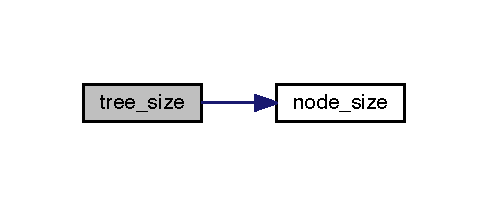
\includegraphics[width=234pt]{tree_8c_abbd772c62da9bafb66ac5513ee870735_cgraph}
\end{center}
\end{figure}


\hypertarget{tree_8c_a5d8936e5b6a90176fd35f7999a1820b8}{\index{tree.\+c@{tree.\+c}!tree\+\_\+traversal@{tree\+\_\+traversal}}
\index{tree\+\_\+traversal@{tree\+\_\+traversal}!tree.\+c@{tree.\+c}}
\subsubsection[{tree\+\_\+traversal}]{\setlength{\rightskip}{0pt plus 5cm}void tree\+\_\+traversal (
\begin{DoxyParamCaption}
\item[{enum {\bf order}}]{order, }
\item[{{\bf tree\+\_\+s} $\ast$}]{tree, }
\item[{{\bf apply\+\_\+f}}]{operation, }
\item[{void $\ast$}]{fst\+\_\+arg}
\end{DoxyParamCaption}
)}}\label{tree_8c_a5d8936e5b6a90176fd35f7999a1820b8}
Traverserar trädet i angiven ordningsföljd och utför en operation på varje element. \begin{DoxySeeAlso}{Se även}
enum \hyperlink{tree_8h_a9f4e8630516f3da89537313b4c828759}{order} 

\hyperlink{tree_8h_a9e54f1284e25a3766511292f740cfdf6}{apply\+\_\+f}
\end{DoxySeeAlso}

\begin{DoxyParams}{Parametrar}
{\em order} & traverseringsordningen \\
\hline
{\em tree} & trädet \\
\hline
{\em operation} & operationen som skall utföras på varje element \\
\hline
{\em argument} & till varje operation (skickas som första argument till apply\+\_\+f-\/funktionen om != N\+U\+L\+L) \\
\hline
\end{DoxyParams}


Här är anropnings diagrammet för den här funktionen\+:
\nopagebreak
\begin{figure}[H]
\begin{center}
\leavevmode
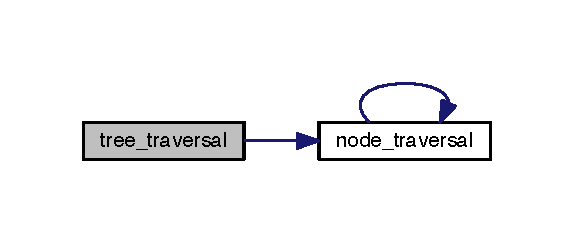
\includegraphics[width=275pt]{tree_8c_a5d8936e5b6a90176fd35f7999a1820b8_cgraph}
\end{center}
\end{figure}



\hypertarget{tree_8h}{\section{tree/tree.h filreferens}
\label{tree_8h}\index{tree/tree.\+h@{tree/tree.\+h}}
}
{\ttfamily \#include $<$stdint.\+h$>$}\\*
{\ttfamily \#include $<$stdbool.\+h$>$}\\*
Include-\/beroendediagram för tree.\+h\+:
\nopagebreak
\begin{figure}[H]
\begin{center}
\leavevmode
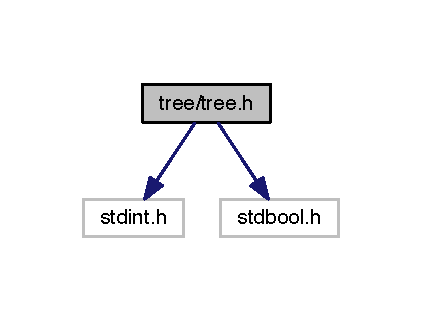
\includegraphics[width=202pt]{tree_8h__incl}
\end{center}
\end{figure}
Den här grafen visar vilka filer som direkt eller indirekt inkluderar denna filen.
\nopagebreak
\begin{figure}[H]
\begin{center}
\leavevmode
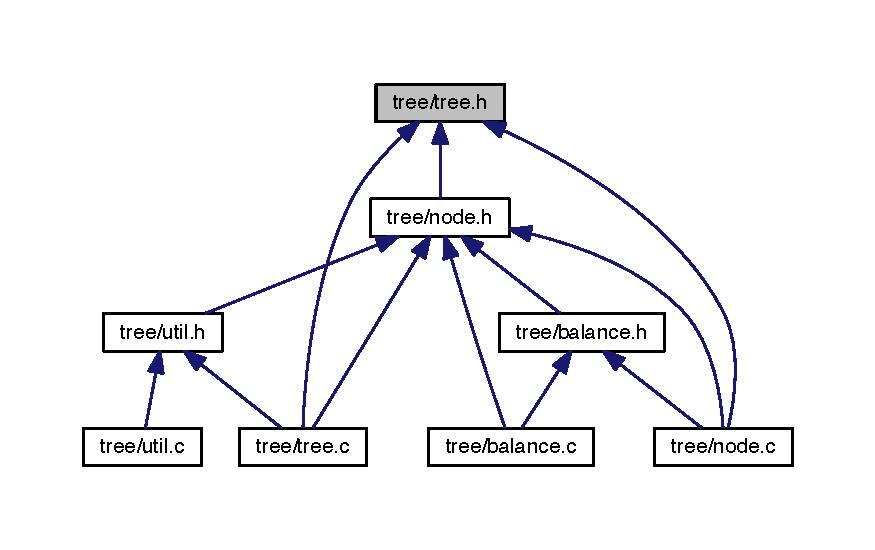
\includegraphics[width=350pt]{tree_8h__dep__incl}
\end{center}
\end{figure}
\subsection*{Typdefinitioner}
\begin{DoxyCompactItemize}
\item 
typedef struct \hyperlink{structtree}{tree} \hyperlink{tree_8h_a563df572fa7aabc17e5f9981cd99460b}{tree\+\_\+s}
\begin{DoxyCompactList}\small\item\em Trädet. \end{DoxyCompactList}\item 
typedef int($\ast$ \hyperlink{tree_8h_ac9404bce0090a72ec95c26c1fc58e4dd}{cmp\+\_\+f} )(void $\ast$, void $\ast$)
\begin{DoxyCompactList}\small\item\em En jämförelsefunktion som används av trädet för att jämföra element. \end{DoxyCompactList}\item 
typedef void($\ast$ \hyperlink{tree_8h_a9e54f1284e25a3766511292f740cfdf6}{apply\+\_\+f} )(void $\ast$, void $\ast$)
\begin{DoxyCompactList}\small\item\em Signaturen för funktioner som skickas som argument till tree\+\_\+traversal. \end{DoxyCompactList}\end{DoxyCompactItemize}
\subsection*{Egenuppräknande typer}
\begin{DoxyCompactItemize}
\item 
enum \hyperlink{tree_8h_a9f4e8630516f3da89537313b4c828759}{order} \{ \hyperlink{tree_8h_a9f4e8630516f3da89537313b4c828759a689aa9fa926510a42fc190e81c65e794}{I\+N\+\_\+\+O\+R\+D\+E\+R}, 
\hyperlink{tree_8h_a9f4e8630516f3da89537313b4c828759a165bf1eccc05929bf679fe6635bc1f2f}{P\+R\+E\+\_\+\+O\+R\+D\+E\+R}, 
\hyperlink{tree_8h_a9f4e8630516f3da89537313b4c828759adb0b29d4ea7b25dfccdef57ec4275e91}{P\+O\+S\+T\+\_\+\+O\+R\+D\+E\+R}
 \}
\begin{DoxyCompactList}\small\item\em Specificerar en traverseringordning. \end{DoxyCompactList}\end{DoxyCompactItemize}
\subsection*{Funktioner}
\begin{DoxyCompactItemize}
\item 
\hyperlink{tree_8h_a563df572fa7aabc17e5f9981cd99460b}{tree\+\_\+s} $\ast$ \hyperlink{tree_8h_ac8974d0f4d710bd6df10d8e38fa0d243}{tree\+\_\+new} (\hyperlink{tree_8h_ac9404bce0090a72ec95c26c1fc58e4dd}{cmp\+\_\+f} key\+\_\+compare\+\_\+function, bool auto\+\_\+balance)
\item 
void \hyperlink{tree_8h_a7ab993db42bc345a1c64e50ba94a8073}{tree\+\_\+delete} (\hyperlink{tree_8h_a563df572fa7aabc17e5f9981cd99460b}{tree\+\_\+s} $\ast$\hyperlink{structtree}{tree})
\item 
void \hyperlink{tree_8h_abc16c36d24d481047dcb82b7cfd6a3a2}{tree\+\_\+insert} (\hyperlink{tree_8h_a563df572fa7aabc17e5f9981cd99460b}{tree\+\_\+s} $\ast$\hyperlink{structtree}{tree}, void $\ast$key, void $\ast$value)
\item 
void \hyperlink{tree_8h_adc1ae204ca89e92d85d8b05878708e72}{tree\+\_\+traversal} (enum \hyperlink{tree_8h_a9f4e8630516f3da89537313b4c828759}{order} \hyperlink{tree_8h_a9f4e8630516f3da89537313b4c828759}{order}, \hyperlink{tree_8h_a563df572fa7aabc17e5f9981cd99460b}{tree\+\_\+s} $\ast$\hyperlink{structtree}{tree}, \hyperlink{tree_8h_a9e54f1284e25a3766511292f740cfdf6}{apply\+\_\+f} operation, void $\ast$fst\+\_\+arg)
\item 
uint32\+\_\+t \hyperlink{tree_8h_a41f3b7564a5da77967a40e2f484e73a8}{tree\+\_\+depth} (\hyperlink{tree_8h_a563df572fa7aabc17e5f9981cd99460b}{tree\+\_\+s} $\ast$\hyperlink{structtree}{tree})
\item 
uint32\+\_\+t \hyperlink{tree_8h_a1c9d41a0f10a772536b25cbf7b992c7a}{tree\+\_\+size} (\hyperlink{tree_8h_a563df572fa7aabc17e5f9981cd99460b}{tree\+\_\+s} $\ast$\hyperlink{structtree}{tree})
\item 
void $\ast$ \hyperlink{tree_8h_a04460bd7f2b87e31e348d2edb8e319ad}{tree\+\_\+get} (\hyperlink{tree_8h_a563df572fa7aabc17e5f9981cd99460b}{tree\+\_\+s} $\ast$\hyperlink{structtree}{tree}, void $\ast$key)
\item 
void $\ast$ \hyperlink{tree_8h_a514ba09f4354c73460494f050e2486cd}{tree\+\_\+remove} (\hyperlink{tree_8h_a563df572fa7aabc17e5f9981cd99460b}{tree\+\_\+s} $\ast$\hyperlink{structtree}{tree}, void $\ast$key)
\item 
char $\ast$ \hyperlink{tree_8h_a369c98a5f5d270aec0725a3367a6122b}{tree\+\_\+get\+\_\+path\+\_\+for\+\_\+element} (\hyperlink{tree_8h_a563df572fa7aabc17e5f9981cd99460b}{tree\+\_\+s} $\ast$\hyperlink{structtree}{tree}, void $\ast$key)
\item 
void $\ast$ \hyperlink{tree_8h_a52252cb35bca876e9e88c10771f72214}{tree\+\_\+get\+\_\+element\+\_\+for\+\_\+path} (\hyperlink{tree_8h_a563df572fa7aabc17e5f9981cd99460b}{tree\+\_\+s} $\ast$\hyperlink{structtree}{tree}, char $\ast$path)
\end{DoxyCompactItemize}


\subsection{Dokumentation över typdefinitioner}
\hypertarget{tree_8h_a9e54f1284e25a3766511292f740cfdf6}{\index{tree.\+h@{tree.\+h}!apply\+\_\+f@{apply\+\_\+f}}
\index{apply\+\_\+f@{apply\+\_\+f}!tree.\+h@{tree.\+h}}
\subsubsection[{apply\+\_\+f}]{\setlength{\rightskip}{0pt plus 5cm}typedef void($\ast$ apply\+\_\+f)(void $\ast$, void $\ast$)}}\label{tree_8h_a9e54f1284e25a3766511292f740cfdf6}


Signaturen för funktioner som skickas som argument till tree\+\_\+traversal. 

\begin{DoxySeeAlso}{Se även}
\hyperlink{tree_8h_adc1ae204ca89e92d85d8b05878708e72}{tree\+\_\+traversal} 
\end{DoxySeeAlso}
\hypertarget{tree_8h_ac9404bce0090a72ec95c26c1fc58e4dd}{\index{tree.\+h@{tree.\+h}!cmp\+\_\+f@{cmp\+\_\+f}}
\index{cmp\+\_\+f@{cmp\+\_\+f}!tree.\+h@{tree.\+h}}
\subsubsection[{cmp\+\_\+f}]{\setlength{\rightskip}{0pt plus 5cm}typedef int($\ast$ cmp\+\_\+f)(void $\ast$, void $\ast$)}}\label{tree_8h_ac9404bce0090a72ec95c26c1fc58e4dd}


En jämförelsefunktion som används av trädet för att jämföra element. 

\hypertarget{tree_8h_a563df572fa7aabc17e5f9981cd99460b}{\index{tree.\+h@{tree.\+h}!tree\+\_\+s@{tree\+\_\+s}}
\index{tree\+\_\+s@{tree\+\_\+s}!tree.\+h@{tree.\+h}}
\subsubsection[{tree\+\_\+s}]{\setlength{\rightskip}{0pt plus 5cm}typedef struct {\bf tree} {\bf tree\+\_\+s}}}\label{tree_8h_a563df572fa7aabc17e5f9981cd99460b}


Trädet. 



\subsection{Dokumentation över egenuppräknande typer}
\hypertarget{tree_8h_a9f4e8630516f3da89537313b4c828759}{\index{tree.\+h@{tree.\+h}!order@{order}}
\index{order@{order}!tree.\+h@{tree.\+h}}
\subsubsection[{order}]{\setlength{\rightskip}{0pt plus 5cm}enum {\bf order}}}\label{tree_8h_a9f4e8630516f3da89537313b4c828759}


Specificerar en traverseringordning. 

\begin{DoxySeeAlso}{Se även}
\hyperlink{tree_8h_adc1ae204ca89e92d85d8b05878708e72}{tree\+\_\+traversal} 
\end{DoxySeeAlso}
\begin{Desc}
\item[Egenuppräknade typers värden]\par
\begin{description}
\index{I\+N\+\_\+\+O\+R\+D\+E\+R@{I\+N\+\_\+\+O\+R\+D\+E\+R}!tree.\+h@{tree.\+h}}\index{tree.\+h@{tree.\+h}!I\+N\+\_\+\+O\+R\+D\+E\+R@{I\+N\+\_\+\+O\+R\+D\+E\+R}}\item[{\em 
\hypertarget{tree_8h_a9f4e8630516f3da89537313b4c828759a689aa9fa926510a42fc190e81c65e794}{I\+N\+\_\+\+O\+R\+D\+E\+R}\label{tree_8h_a9f4e8630516f3da89537313b4c828759a689aa9fa926510a42fc190e81c65e794}
}]\index{P\+R\+E\+\_\+\+O\+R\+D\+E\+R@{P\+R\+E\+\_\+\+O\+R\+D\+E\+R}!tree.\+h@{tree.\+h}}\index{tree.\+h@{tree.\+h}!P\+R\+E\+\_\+\+O\+R\+D\+E\+R@{P\+R\+E\+\_\+\+O\+R\+D\+E\+R}}\item[{\em 
\hypertarget{tree_8h_a9f4e8630516f3da89537313b4c828759a165bf1eccc05929bf679fe6635bc1f2f}{P\+R\+E\+\_\+\+O\+R\+D\+E\+R}\label{tree_8h_a9f4e8630516f3da89537313b4c828759a165bf1eccc05929bf679fe6635bc1f2f}
}]\index{P\+O\+S\+T\+\_\+\+O\+R\+D\+E\+R@{P\+O\+S\+T\+\_\+\+O\+R\+D\+E\+R}!tree.\+h@{tree.\+h}}\index{tree.\+h@{tree.\+h}!P\+O\+S\+T\+\_\+\+O\+R\+D\+E\+R@{P\+O\+S\+T\+\_\+\+O\+R\+D\+E\+R}}\item[{\em 
\hypertarget{tree_8h_a9f4e8630516f3da89537313b4c828759adb0b29d4ea7b25dfccdef57ec4275e91}{P\+O\+S\+T\+\_\+\+O\+R\+D\+E\+R}\label{tree_8h_a9f4e8630516f3da89537313b4c828759adb0b29d4ea7b25dfccdef57ec4275e91}
}]\end{description}
\end{Desc}


\subsection{Dokumentation över funktioner}
\hypertarget{tree_8h_a7ab993db42bc345a1c64e50ba94a8073}{\index{tree.\+h@{tree.\+h}!tree\+\_\+delete@{tree\+\_\+delete}}
\index{tree\+\_\+delete@{tree\+\_\+delete}!tree.\+h@{tree.\+h}}
\subsubsection[{tree\+\_\+delete}]{\setlength{\rightskip}{0pt plus 5cm}void tree\+\_\+delete (
\begin{DoxyParamCaption}
\item[{{\bf tree\+\_\+s} $\ast$}]{tree}
\end{DoxyParamCaption}
)}}\label{tree_8h_a7ab993db42bc345a1c64e50ba94a8073}
Ta bort trädet ur minnes.


\begin{DoxyParams}{Parametrar}
{\em tree} & trädet\\
\hline
\end{DoxyParams}
Sorteringsnycklar och element tas inte bort ur minnet. 

Här är anropnings diagrammet för den här funktionen\+:
\nopagebreak
\begin{figure}[H]
\begin{center}
\leavevmode
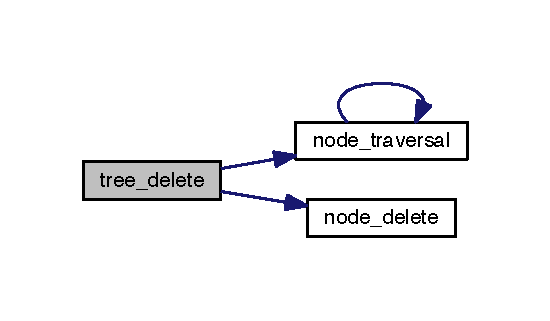
\includegraphics[width=264pt]{tree_8h_a7ab993db42bc345a1c64e50ba94a8073_cgraph}
\end{center}
\end{figure}


\hypertarget{tree_8h_a41f3b7564a5da77967a40e2f484e73a8}{\index{tree.\+h@{tree.\+h}!tree\+\_\+depth@{tree\+\_\+depth}}
\index{tree\+\_\+depth@{tree\+\_\+depth}!tree.\+h@{tree.\+h}}
\subsubsection[{tree\+\_\+depth}]{\setlength{\rightskip}{0pt plus 5cm}uint32\+\_\+t tree\+\_\+depth (
\begin{DoxyParamCaption}
\item[{{\bf tree\+\_\+s} $\ast$}]{tree}
\end{DoxyParamCaption}
)}}\label{tree_8h_a41f3b7564a5da77967a40e2f484e73a8}
Returnerar djupet i trädet.


\begin{DoxyParams}{Parametrar}
{\em tree} & trädet \\
\hline
\end{DoxyParams}
\begin{DoxyReturn}{Returnerar}
tree\+:s djup 
\end{DoxyReturn}


Här är anropnings diagrammet för den här funktionen\+:
\nopagebreak
\begin{figure}[H]
\begin{center}
\leavevmode
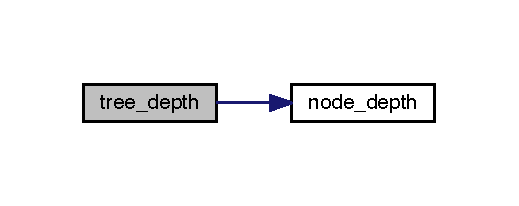
\includegraphics[width=249pt]{tree_8h_a41f3b7564a5da77967a40e2f484e73a8_cgraph}
\end{center}
\end{figure}




Här är katalog-\/grafen för denna funktion\+:
\nopagebreak
\begin{figure}[H]
\begin{center}
\leavevmode
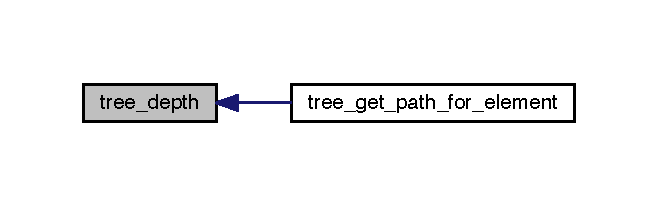
\includegraphics[width=316pt]{tree_8h_a41f3b7564a5da77967a40e2f484e73a8_icgraph}
\end{center}
\end{figure}


\hypertarget{tree_8h_a04460bd7f2b87e31e348d2edb8e319ad}{\index{tree.\+h@{tree.\+h}!tree\+\_\+get@{tree\+\_\+get}}
\index{tree\+\_\+get@{tree\+\_\+get}!tree.\+h@{tree.\+h}}
\subsubsection[{tree\+\_\+get}]{\setlength{\rightskip}{0pt plus 5cm}void$\ast$ tree\+\_\+get (
\begin{DoxyParamCaption}
\item[{{\bf tree\+\_\+s} $\ast$}]{tree, }
\item[{void $\ast$}]{key}
\end{DoxyParamCaption}
)}}\label{tree_8h_a04460bd7f2b87e31e348d2edb8e319ad}
Returnerar en pekare till ett element i trädet.


\begin{DoxyParams}{Parametrar}
{\em tree} & trädet \\
\hline
{\em key} & sorteringsnyckeln för det sökta elementet \\
\hline
\end{DoxyParams}
\begin{DoxyReturn}{Returnerar}
det matchande elementet från trädet 
\end{DoxyReturn}
\hypertarget{tree_8h_a52252cb35bca876e9e88c10771f72214}{\index{tree.\+h@{tree.\+h}!tree\+\_\+get\+\_\+element\+\_\+for\+\_\+path@{tree\+\_\+get\+\_\+element\+\_\+for\+\_\+path}}
\index{tree\+\_\+get\+\_\+element\+\_\+for\+\_\+path@{tree\+\_\+get\+\_\+element\+\_\+for\+\_\+path}!tree.\+h@{tree.\+h}}
\subsubsection[{tree\+\_\+get\+\_\+element\+\_\+for\+\_\+path}]{\setlength{\rightskip}{0pt plus 5cm}void$\ast$ tree\+\_\+get\+\_\+element\+\_\+for\+\_\+path (
\begin{DoxyParamCaption}
\item[{{\bf tree\+\_\+s} $\ast$}]{tree, }
\item[{char $\ast$}]{path}
\end{DoxyParamCaption}
)}}\label{tree_8h_a52252cb35bca876e9e88c10771f72214}
Tar en sträng med samma format som returneras från tree\+\_\+get\+\_\+path\+\_\+for\+\_\+element och returnerar elementet på den platsen i trädet.


\begin{DoxyParams}{Parametrar}
{\em tree} & trädet \\
\hline
{\em path} & pathen till elementet som skall returneras \\
\hline
\end{DoxyParams}
\begin{DoxyReturn}{Returnerar}
en pekare till ett element eller N\+U\+L\+L 
\end{DoxyReturn}
\hypertarget{tree_8h_a369c98a5f5d270aec0725a3367a6122b}{\index{tree.\+h@{tree.\+h}!tree\+\_\+get\+\_\+path\+\_\+for\+\_\+element@{tree\+\_\+get\+\_\+path\+\_\+for\+\_\+element}}
\index{tree\+\_\+get\+\_\+path\+\_\+for\+\_\+element@{tree\+\_\+get\+\_\+path\+\_\+for\+\_\+element}!tree.\+h@{tree.\+h}}
\subsubsection[{tree\+\_\+get\+\_\+path\+\_\+for\+\_\+element}]{\setlength{\rightskip}{0pt plus 5cm}char$\ast$ tree\+\_\+get\+\_\+path\+\_\+for\+\_\+element (
\begin{DoxyParamCaption}
\item[{{\bf tree\+\_\+s} $\ast$}]{tree, }
\item[{void $\ast$}]{key}
\end{DoxyParamCaption}
)}}\label{tree_8h_a369c98a5f5d270aec0725a3367a6122b}
Returnerar en path till ett element i trädet.

En path kan vara t.\+ex. \char`\"{}\char`\"{} för roten, \char`\"{}\+L\+L\char`\"{} för två steg vänster, \char`\"{}\+L\+R\char`\"{} för vänster-\/höger etc.


\begin{DoxyParams}{Parametrar}
{\em tree} & trädet \\
\hline
{\em key} & sorteringsnyckeln för det sökta elementet \\
\hline
\end{DoxyParams}
\begin{DoxyReturn}{Returnerar}
pathen till el, ev N\+U\+L\+L om el inte finns i trädet 
\end{DoxyReturn}


Här är anropnings diagrammet för den här funktionen\+:
\nopagebreak
\begin{figure}[H]
\begin{center}
\leavevmode
\includegraphics[width=350pt]{tree_8h_a369c98a5f5d270aec0725a3367a6122b_cgraph}
\end{center}
\end{figure}


\hypertarget{tree_8h_abc16c36d24d481047dcb82b7cfd6a3a2}{\index{tree.\+h@{tree.\+h}!tree\+\_\+insert@{tree\+\_\+insert}}
\index{tree\+\_\+insert@{tree\+\_\+insert}!tree.\+h@{tree.\+h}}
\subsubsection[{tree\+\_\+insert}]{\setlength{\rightskip}{0pt plus 5cm}void tree\+\_\+insert (
\begin{DoxyParamCaption}
\item[{{\bf tree\+\_\+s} $\ast$}]{tree, }
\item[{void $\ast$}]{key, }
\item[{void $\ast$}]{value}
\end{DoxyParamCaption}
)}}\label{tree_8h_abc16c36d24d481047dcb82b7cfd6a3a2}
Stoppar in ett element i trädet.

O\+B\+S! Implementationen förutsätter att alla nycklar är unika vid insättning!


\begin{DoxyParams}{Parametrar}
{\em tree} & trädet \\
\hline
{\em key} & sorteringsnyckeln för elementet \\
\hline
{\em value} & elementet som skall stoppas in \\
\hline
\end{DoxyParams}


Här är anropnings diagrammet för den här funktionen\+:
\nopagebreak
\begin{figure}[H]
\begin{center}
\leavevmode
\includegraphics[width=350pt]{tree_8h_abc16c36d24d481047dcb82b7cfd6a3a2_cgraph}
\end{center}
\end{figure}


\hypertarget{tree_8h_ac8974d0f4d710bd6df10d8e38fa0d243}{\index{tree.\+h@{tree.\+h}!tree\+\_\+new@{tree\+\_\+new}}
\index{tree\+\_\+new@{tree\+\_\+new}!tree.\+h@{tree.\+h}}
\subsubsection[{tree\+\_\+new}]{\setlength{\rightskip}{0pt plus 5cm}{\bf tree\+\_\+s}$\ast$ tree\+\_\+new (
\begin{DoxyParamCaption}
\item[{{\bf cmp\+\_\+f}}]{key\+\_\+compare\+\_\+function, }
\item[{bool}]{auto\+\_\+balance}
\end{DoxyParamCaption}
)}}\label{tree_8h_ac8974d0f4d710bd6df10d8e38fa0d243}
Skapa ett nytt träd.


\begin{DoxyParams}{Parametrar}
{\em key\+\_\+compare\+\_\+function} & pekar ut den jämförelsefunktion som skall användas för att jämföra elementen i trädet \\
\hline
{\em auto\+\_\+balance} & är true om trädet skall balansera sig automatiskt vid insättning och borttagning\\
\hline
\end{DoxyParams}
Jämförelsefunktionen skall fungera som strcmp map returvärden. \hypertarget{tree_8h_a514ba09f4354c73460494f050e2486cd}{\index{tree.\+h@{tree.\+h}!tree\+\_\+remove@{tree\+\_\+remove}}
\index{tree\+\_\+remove@{tree\+\_\+remove}!tree.\+h@{tree.\+h}}
\subsubsection[{tree\+\_\+remove}]{\setlength{\rightskip}{0pt plus 5cm}void$\ast$ tree\+\_\+remove (
\begin{DoxyParamCaption}
\item[{{\bf tree\+\_\+s} $\ast$}]{tree, }
\item[{void $\ast$}]{key}
\end{DoxyParamCaption}
)}}\label{tree_8h_a514ba09f4354c73460494f050e2486cd}
Tar bort ett element ur trädet.


\begin{DoxyParams}{Parametrar}
{\em tree} & trädet \\
\hline
{\em key} & sorteringsnyckeln för det sökta elementet \\
\hline
\end{DoxyParams}
\begin{DoxyReturn}{Returnerar}
en pekare till elementet eller N\+U\+L\+L om det inte fanns i trädet 
\end{DoxyReturn}


Här är anropnings diagrammet för den här funktionen\+:
\nopagebreak
\begin{figure}[H]
\begin{center}
\leavevmode
\includegraphics[width=350pt]{tree_8h_a514ba09f4354c73460494f050e2486cd_cgraph}
\end{center}
\end{figure}


\hypertarget{tree_8h_a1c9d41a0f10a772536b25cbf7b992c7a}{\index{tree.\+h@{tree.\+h}!tree\+\_\+size@{tree\+\_\+size}}
\index{tree\+\_\+size@{tree\+\_\+size}!tree.\+h@{tree.\+h}}
\subsubsection[{tree\+\_\+size}]{\setlength{\rightskip}{0pt plus 5cm}uint32\+\_\+t tree\+\_\+size (
\begin{DoxyParamCaption}
\item[{{\bf tree\+\_\+s} $\ast$}]{tree}
\end{DoxyParamCaption}
)}}\label{tree_8h_a1c9d41a0f10a772536b25cbf7b992c7a}
Returnerar trädets storlek (antalet noder).


\begin{DoxyParams}{Parametrar}
{\em tree} & trädet \\
\hline
\end{DoxyParams}
\begin{DoxyReturn}{Returnerar}
tree\+:s storlek (antalet noder) 
\end{DoxyReturn}


Här är anropnings diagrammet för den här funktionen\+:
\nopagebreak
\begin{figure}[H]
\begin{center}
\leavevmode
\includegraphics[width=234pt]{tree_8h_a1c9d41a0f10a772536b25cbf7b992c7a_cgraph}
\end{center}
\end{figure}


\hypertarget{tree_8h_adc1ae204ca89e92d85d8b05878708e72}{\index{tree.\+h@{tree.\+h}!tree\+\_\+traversal@{tree\+\_\+traversal}}
\index{tree\+\_\+traversal@{tree\+\_\+traversal}!tree.\+h@{tree.\+h}}
\subsubsection[{tree\+\_\+traversal}]{\setlength{\rightskip}{0pt plus 5cm}void tree\+\_\+traversal (
\begin{DoxyParamCaption}
\item[{enum {\bf order}}]{order, }
\item[{{\bf tree\+\_\+s} $\ast$}]{tree, }
\item[{{\bf apply\+\_\+f}}]{operation, }
\item[{void $\ast$}]{fst\+\_\+arg}
\end{DoxyParamCaption}
)}}\label{tree_8h_adc1ae204ca89e92d85d8b05878708e72}
Traverserar trädet i angiven ordningsföljd och utför en operation på varje element. \begin{DoxySeeAlso}{Se även}
enum \hyperlink{tree_8h_a9f4e8630516f3da89537313b4c828759}{order} 

\hyperlink{tree_8h_a9e54f1284e25a3766511292f740cfdf6}{apply\+\_\+f}
\end{DoxySeeAlso}

\begin{DoxyParams}{Parametrar}
{\em order} & traverseringsordningen \\
\hline
{\em tree} & trädet \\
\hline
{\em operation} & operationen som skall utföras på varje element \\
\hline
{\em argument} & till varje operation (skickas som första argument till apply\+\_\+f-\/funktionen om != N\+U\+L\+L) \\
\hline
\end{DoxyParams}


Här är anropnings diagrammet för den här funktionen\+:
\nopagebreak
\begin{figure}[H]
\begin{center}
\leavevmode
\includegraphics[width=275pt]{tree_8h_adc1ae204ca89e92d85d8b05878708e72_cgraph}
\end{center}
\end{figure}



\hypertarget{util_8c}{\section{tree/util.c filreferens}
\label{util_8c}\index{tree/util.\+c@{tree/util.\+c}}
}
{\ttfamily \#include \char`\"{}util.\+h\char`\"{}}\\*
Include-\/beroendediagram för util.\+c\+:
\nopagebreak
\begin{figure}[H]
\begin{center}
\leavevmode
\includegraphics[width=225pt]{util_8c__incl}
\end{center}
\end{figure}
\subsection*{Definitioner}
\begin{DoxyCompactItemize}
\item 
\#define \hyperlink{util_8c_a4886a8f966a69949cefc46a6a3468006}{Max}(a, b)~(a $<$ b ? b \+: a)
\end{DoxyCompactItemize}
\subsection*{Funktioner}
\begin{DoxyCompactItemize}
\item 
uint32\+\_\+t \hyperlink{util_8c_a3934222d89b56dbe6612d3128f9fe4da}{node\+\_\+depth} (\hyperlink{node_8h_aeed67813c57d1b99aba54f16aa01639f}{node\+\_\+s} $\ast$n)
\begin{DoxyCompactList}\small\item\em Returnerar subträdets djup. \end{DoxyCompactList}\item 
uint32\+\_\+t \hyperlink{util_8c_ac334fa878f7aa93d140875390c4eed10}{node\+\_\+size} (\hyperlink{node_8h_aeed67813c57d1b99aba54f16aa01639f}{node\+\_\+s} $\ast$n)
\begin{DoxyCompactList}\small\item\em Returnerar subträdets storlek. \end{DoxyCompactList}\end{DoxyCompactItemize}


\subsection{Dokumentation över definitioner}
\hypertarget{util_8c_a4886a8f966a69949cefc46a6a3468006}{\index{util.\+c@{util.\+c}!Max@{Max}}
\index{Max@{Max}!util.\+c@{util.\+c}}
\subsubsection[{Max}]{\setlength{\rightskip}{0pt plus 5cm}\#define Max(
\begin{DoxyParamCaption}
\item[{}]{a, }
\item[{}]{b}
\end{DoxyParamCaption}
)~(a $<$ b ? b \+: a)}}\label{util_8c_a4886a8f966a69949cefc46a6a3468006}


\subsection{Dokumentation över funktioner}
\hypertarget{util_8c_a3934222d89b56dbe6612d3128f9fe4da}{\index{util.\+c@{util.\+c}!node\+\_\+depth@{node\+\_\+depth}}
\index{node\+\_\+depth@{node\+\_\+depth}!util.\+c@{util.\+c}}
\subsubsection[{node\+\_\+depth}]{\setlength{\rightskip}{0pt plus 5cm}uint32\+\_\+t node\+\_\+depth (
\begin{DoxyParamCaption}
\item[{{\bf node\+\_\+s} $\ast$}]{n}
\end{DoxyParamCaption}
)}}\label{util_8c_a3934222d89b56dbe6612d3128f9fe4da}


Returnerar subträdets djup. 

\begin{DoxySeeAlso}{Se även}
\hyperlink{tree_8h_a41f3b7564a5da77967a40e2f484e73a8}{tree\+\_\+depth} 
\end{DoxySeeAlso}


Här är anropnings diagrammet för den här funktionen\+:
\nopagebreak
\begin{figure}[H]
\begin{center}
\leavevmode
\includegraphics[width=149pt]{util_8c_a3934222d89b56dbe6612d3128f9fe4da_cgraph}
\end{center}
\end{figure}




Här är katalog-\/grafen för denna funktion\+:
\nopagebreak
\begin{figure}[H]
\begin{center}
\leavevmode
\includegraphics[width=350pt]{util_8c_a3934222d89b56dbe6612d3128f9fe4da_icgraph}
\end{center}
\end{figure}


\hypertarget{util_8c_ac334fa878f7aa93d140875390c4eed10}{\index{util.\+c@{util.\+c}!node\+\_\+size@{node\+\_\+size}}
\index{node\+\_\+size@{node\+\_\+size}!util.\+c@{util.\+c}}
\subsubsection[{node\+\_\+size}]{\setlength{\rightskip}{0pt plus 5cm}uint32\+\_\+t node\+\_\+size (
\begin{DoxyParamCaption}
\item[{{\bf node\+\_\+s} $\ast$}]{n}
\end{DoxyParamCaption}
)}}\label{util_8c_ac334fa878f7aa93d140875390c4eed10}


Returnerar subträdets storlek. 

\begin{DoxySeeAlso}{Se även}
\hyperlink{tree_8h_a1c9d41a0f10a772536b25cbf7b992c7a}{tree\+\_\+size} 
\end{DoxySeeAlso}


Här är anropnings diagrammet för den här funktionen\+:
\nopagebreak
\begin{figure}[H]
\begin{center}
\leavevmode
\includegraphics[width=142pt]{util_8c_ac334fa878f7aa93d140875390c4eed10_cgraph}
\end{center}
\end{figure}




Här är katalog-\/grafen för denna funktion\+:
\nopagebreak
\begin{figure}[H]
\begin{center}
\leavevmode
\includegraphics[width=239pt]{util_8c_ac334fa878f7aa93d140875390c4eed10_icgraph}
\end{center}
\end{figure}



\hypertarget{util_8h}{\section{tree/util.h filreferens}
\label{util_8h}\index{tree/util.\+h@{tree/util.\+h}}
}
{\ttfamily \#include $<$stdint.\+h$>$}\\*
{\ttfamily \#include \char`\"{}node.\+h\char`\"{}}\\*
Include-\/beroendediagram för util.\+h\+:
\nopagebreak
\begin{figure}[H]
\begin{center}
\leavevmode
\includegraphics[width=225pt]{util_8h__incl}
\end{center}
\end{figure}
Den här grafen visar vilka filer som direkt eller indirekt inkluderar denna filen.
\nopagebreak
\begin{figure}[H]
\begin{center}
\leavevmode
\includegraphics[width=216pt]{util_8h__dep__incl}
\end{center}
\end{figure}
\subsection*{Funktioner}
\begin{DoxyCompactItemize}
\item 
uint32\+\_\+t \hyperlink{util_8h_a3934222d89b56dbe6612d3128f9fe4da}{node\+\_\+depth} (\hyperlink{node_8h_aeed67813c57d1b99aba54f16aa01639f}{node\+\_\+s} $\ast$n)
\begin{DoxyCompactList}\small\item\em Returnerar subträdets djup. \end{DoxyCompactList}\item 
uint32\+\_\+t \hyperlink{util_8h_ac334fa878f7aa93d140875390c4eed10}{node\+\_\+size} (\hyperlink{node_8h_aeed67813c57d1b99aba54f16aa01639f}{node\+\_\+s} $\ast$n)
\begin{DoxyCompactList}\small\item\em Returnerar subträdets storlek. \end{DoxyCompactList}\end{DoxyCompactItemize}


\subsection{Dokumentation över funktioner}
\hypertarget{util_8h_a3934222d89b56dbe6612d3128f9fe4da}{\index{util.\+h@{util.\+h}!node\+\_\+depth@{node\+\_\+depth}}
\index{node\+\_\+depth@{node\+\_\+depth}!util.\+h@{util.\+h}}
\subsubsection[{node\+\_\+depth}]{\setlength{\rightskip}{0pt plus 5cm}uint32\+\_\+t node\+\_\+depth (
\begin{DoxyParamCaption}
\item[{{\bf node\+\_\+s} $\ast$}]{n}
\end{DoxyParamCaption}
)}}\label{util_8h_a3934222d89b56dbe6612d3128f9fe4da}


Returnerar subträdets djup. 

\begin{DoxySeeAlso}{Se även}
\hyperlink{tree_8h_a41f3b7564a5da77967a40e2f484e73a8}{tree\+\_\+depth} 
\end{DoxySeeAlso}


Här är anropnings diagrammet för den här funktionen\+:
\nopagebreak
\begin{figure}[H]
\begin{center}
\leavevmode
\includegraphics[width=254pt]{util_8h_a3934222d89b56dbe6612d3128f9fe4da_cgraph}
\end{center}
\end{figure}




Här är katalog-\/grafen för denna funktion\+:
\nopagebreak
\begin{figure}[H]
\begin{center}
\leavevmode
\includegraphics[width=149pt]{util_8h_a3934222d89b56dbe6612d3128f9fe4da_icgraph}
\end{center}
\end{figure}


\hypertarget{util_8h_ac334fa878f7aa93d140875390c4eed10}{\index{util.\+h@{util.\+h}!node\+\_\+size@{node\+\_\+size}}
\index{node\+\_\+size@{node\+\_\+size}!util.\+h@{util.\+h}}
\subsubsection[{node\+\_\+size}]{\setlength{\rightskip}{0pt plus 5cm}uint32\+\_\+t node\+\_\+size (
\begin{DoxyParamCaption}
\item[{{\bf node\+\_\+s} $\ast$}]{n}
\end{DoxyParamCaption}
)}}\label{util_8h_ac334fa878f7aa93d140875390c4eed10}


Returnerar subträdets storlek. 

\begin{DoxySeeAlso}{Se även}
\hyperlink{tree_8h_a1c9d41a0f10a772536b25cbf7b992c7a}{tree\+\_\+size} 
\end{DoxySeeAlso}


Här är anropnings diagrammet för den här funktionen\+:
\nopagebreak
\begin{figure}[H]
\begin{center}
\leavevmode
\includegraphics[width=239pt]{util_8h_ac334fa878f7aa93d140875390c4eed10_cgraph}
\end{center}
\end{figure}




Här är katalog-\/grafen för denna funktion\+:
\nopagebreak
\begin{figure}[H]
\begin{center}
\leavevmode
\includegraphics[width=142pt]{util_8h_ac334fa878f7aa93d140875390c4eed10_icgraph}
\end{center}
\end{figure}



%--- End generated contents ---

% Index
\newpage
\phantomsection
\addcontentsline{toc}{chapter}{Index}
\printindex

\end{document}
